% !TEX options=--shell-escape
\documentclass[a4paper,12pt, oneside]{book}
\usepackage[utf8]{inputenc}
\usepackage[T1]{fontenc}
\usepackage[spanish]{babel}
\usepackage{a4wide}
\usepackage{graphicx}
\graphicspath{{images/}}
\usepackage{subfig}
\usepackage{tikz}
\usepackage{float}
\usepackage{lscape}
\usetikzlibrary{shapes,arrows}
\usepackage{pgfplots}
\pgfplotsset{compat=newest}
\pgfplotsset{plot coordinates/math parser=false}
\newlength\figureheight
\newlength\figurewidth
\pgfkeys{/pgf/number format/.cd,
set decimal separator={,\!},
1000 sep={\,},
}
\usepackage{ifthen}
\usepackage{ifpdf}
\ifpdf
\usepackage[pdftex]{hyperref}
\else
\usepackage{hyperref}
\fi
\usepackage{color}
\usepackage{longtable}
%\usepackage{minted}
\hypersetup{%
colorlinks=true,
linkcolor=black,
citecolor=black,
urlcolor=black}

\renewcommand{\baselinestretch}{1.05}
\usepackage{fancyhdr}
\pagestyle{fancy}
\fancyfoot{}
\fancyhead[LE,RO]{\bfseries\thepage}
\fancyhead[RE]{\bfseries\nouppercase{\leftmark}}
\fancyhead[LO]{\bfseries\nouppercase{\rightmark}}
\setlength{\headheight}{15pt}

\let\headruleORIG\headrule
\renewcommand{\headrule}{\color{black} \headruleORIG}
\renewcommand{\headrulewidth}{1.0pt}
\usepackage{colortbl}
\arrayrulecolor{black}

\fancypagestyle{plain}{
  \fancyhead{}
  \fancyfoot[C]{\thepage}
  \renewcommand{\headrulewidth}{0pt}
}

\makeatletter
\def\@textbottom{\vskip \z@ \@plus 1pt}
\let\@texttop\relax
\makeatother

\makeatletter
\def\cleardoublepage{\clearpage\if@twoside \ifodd\c@page\else%
  \hbox{}%
  \thispagestyle{empty}%
  \newpage%
  \if@twocolumn\hbox{}\newpage\fi\fi\fi}
\makeatother

\usepackage{amsthm}
\usepackage{amssymb,amsmath,bbm}
\usepackage{array}
\usepackage{bm}
\usepackage{multirow}
\usepackage[footnote]{acronym}
\usepackage{booktabs}
\usepackage{minted}
\begin{document}

%%%%%%%%%%%%%%%%%%
%%% First page %%%
%%%%%%%%%%%%%%%%%%

\begin{titlepage}
\begin{center}

{\large Máster en Ciencia de Datos e Ingeniería de Computadores.}\\[0.5cm]

{\large \textbf{Asignatura: }Introducción a la Ciencia de Datos}\\[0.5cm]

% Title
\rule{\linewidth}{0.5mm} \\[0.4cm]
{ \huge \bfseries Trabajo teórico/práctico integrador\\[0.4cm] }
\rule{\linewidth}{0.5mm} \\[1.5cm]

\begin{flushright}
Dataset de regresión: \textit{baseball} \\
Dataset de clasificación: \textit{contraceptive} \\
\end{flushright}
% Author and supervisor

\vfill
\begin{flushleft}
\textbf{Autor: } David Criado Ramón.\\
\textbf{D.N.I.: } 26254133-R \\
\textbf{E-mail: } davidcr96@correo.ugr.es \\
\end{flushleft}

% Bottom of the page

\end{center}
\end{titlepage}

%%%%%%%%%%%%%%%%%%%%%%%%%%%%%
%%% Non-significant pages %%%
%%%%%%%%%%%%%%%%%%%%%%%%%%%%%

\frontmatter

\clearpage
\tableofcontents

\clearpage
\listoffigures

\clearpage

%%%%%%%%%%%%%%%%%%%%%%%%%%%%%%%%%%%%%%%%%%%%
%%% Content of the report and references %%%
%%%%%%%%%%%%%%%%%%%%%%%%%%%%%%%%%%%%%%%%%%%%

\mainmatter
\pagestyle{fancy}
\chapter{Análisis Exploratorio de Datos (EDA).}
\section{EDA - dataset de regresión ``baseball''.}
\subsection{Descripción del dataset.}
El dataset ``baseball'' contiene información relativa a los jugadores de béisbol de la MLB \textit{(Major League Baseball)} en la temporada 1991/1992. En concreto, contiene información sobre aquellos jugadores que tenían el rol de bateador, incluyendo varios estadísticos de rendimiento de los jugadores, alguna información extra relativa a la competitividad de su salario (la posibilidad de solicitar un arbitraje o ser agente libre) y el salario que obtuvieron durante esa temporada.

\subsection{Descripción del tipo del dato de entrada.}
Tras leer los datos tenemos un ``data.frame'', con 337 muestras y 17 características. Todas las variables leídas son de tipo numeric (número real). De entre ellas, hay cuatro de carácter categórico \textit{Free\_agency\_eligibility, Free\_agent, Arbitration\_eligibility y Arbitration} con representación binaria cada uno (0/1) que pasaremos durante el proceso de EDA a factores (No/Sí). \textit{Nota: Para la parte de regresión nos será útil la representación binaria planteada inicialmente}.\\

A continuación, vamos a describir de forma breve el significado de cada una de las características, para poder comprender mejor los datos de los que disponemos y poder plantear algunas hipótesis iniciales.

\begin{itemize}
	\item \textbf{Batting\_average} - Es el número de hits dividido por el número de oportunidades al bate.
	\item \textbf{On-base\_percentage} - Mide con que frecuencia un jugador alcanza una base.
	\item \textbf{Runs} - Número de carreras anotadas. Una carrera es similar a un punto en otros deportes. Para anotar una carrera el jugador ha de alcanzar la primera base, segunda, tercera y volver a la base inicial.
	\item \textbf{Hits} - Un hit ocurre cuando un jugador alcanza al menos una base tras realizar un lanzamiento correcto con el bate. Normalmente incluye hits sencillos, dobles, triples y homeruns.
	\item \textbf{Doubles} - Hit doble.
	\item \textbf{Triples} - Hit triple.
	\item \textbf{HomeRuns} - Situación en la que el bateador es capaz de golpear la bola de manera que puede pasar por todas las bases y anotar una carrera en la misma jugada.
	\item \textbf{Runs\_batted\_in} - Se acredita un RBI a un bateador si la jugada que hacer permite anotar una carrera. Por ejemplo, si hace un hit en una base y otro jugador en otra base más avanzada puede anotar la carrera.
	\item \textbf{Walks} - Ocurre cuando el pitcher lanza cuatro bolas fuera de la zona de golpeo. En ese caso, al bateador (que no ha intentado darle a la bola, ha de darse cuenta de la situación) se le garantiza la primera base.
	\item \textbf{Strike-outs} - Es la acumulación de tres \textit{strikes}, elimina al bateador de la jugada. Un \textit{strike} ocurre cuando el bateador no consigue golpear la pelota (pero lo intenta) o el tiro acaba en una situación de juego injusta o inválida.
	\item \textbf{Stolen-bases} - Aparte de cuando la pelota está en juego tras el lanzamiento del bateador, el \textit{runner} (jugador que está en una base y quiere volver a la base inicial para anotar una carrera) puede intentar llegar a otra base mientras la pelota está en juego, habitualmente ocurre mientras el \textit{pitcher} lanza la pelota a la zona de lanzamiento. La defensa puede impedir la jugada llevando la pelota a la base.
	\item \textbf{Errors} - Es cualquier maniobra errónea realizada por un jugador defensivo que permita a un \textit{runner} avanzar una o más bases de las que debería.
	\item \textbf{Free\_agency\_eligibility} - Un jugador es agente libre si él y su equipo finalizan el contrato o llevan más de 6 años como jugadores profesionales en la MLB.
	\item \textbf{Free\_agency} - El jugador fue agente libre en la temporada 91/92.
	\item \textbf{Arbitration\_eligibility} - Un jugador es elegible para solicitar un proceso de arbitración de su salario si lleva más de tres años como jugador profesional en la MLB y menos de seis años. En el proceso de arbitración, el jugador y el equipo al que representan no se ponen de acuerdo para determinar su salario. Así que ambas partes plantean un salario y argumentan para ello y una tercera parte decide cuál de las dos opciones aplicar.
	\item \textbf{Arbitration} - El jugador estuvo implicado en un proceso de arbitración en la temporada 91/92.
	\item \textbf{Salary} - Salario anual que obtuvo el bateador en la temporada 91/92.
\end{itemize}

\subsection{Planteamiento de hipótesis.}
\begin{itemize}
\item El \textit{``homerun''} es una de las jugadas más conocidas del béisbol, ¿está fuertemente relacionado de forma positiva con el salario?
\item En la MLB existen métodos como la arbitración que permiten a un jugador reclamar derechos sobre su salario, ¿está el salario acotado inferior y/o superiormente? En caso positivo, ¿cómo afecta la posibilidad de solicitar arbitración a esas cotas?
\item Dentro de los estadísticos de béisbol que disponemos, tenemos dos de carácter negativo, \textit{strike-outs} para el bateador y \textit{errors} para un jugador defensivo, ¿implica ésto una disminución del salario de los jugadores?
\item Ser agente libre (más de 6 años en la MLB a no ser que se finalice el contrato con el equipo) y disponer de arbitración (entre 3 y 6 años en la MLB), no sólo son mecanismos para mejorar la competitividad del salario de los jugadores, también son indicativos de la veteranía del jugador. ¿Tienen un salario mayor los jugadores más veteranos?
\end{itemize}

\subsection{Cálculo de medidas de tendencia central, dispersión y dominio.}
Para poder analizar a continuación mejor el comportamiento de las variables, vamos a considerar: su valor mínimo y máximo; como valores de tendencia central: la media y la mediana; y como valores de dispersión: desviación estándar y desviación absoluta de la mediana. Los resultados los vamos a poner resumidos en la siguiente tabla (en esta tabla no incluimos las variables categóricas).

\begin{longtable}{@{}c|rrrrrr@{}}
\toprule
\textbf{Nombre} & \multicolumn{1}{c}{\textbf{Min}} & \multicolumn{1}{c}{\textbf{Max}} & \multicolumn{1}{c}{\textbf{Media}} & \multicolumn{1}{c}{\textbf{Mediana}} & \multicolumn{1}{c}{\textbf{\begin{tabular}[c]{@{}c@{}}Desviación \\ estándar\end{tabular}}} & \multicolumn{1}{c}{\textbf{\begin{tabular}[c]{@{}c@{}}Desviación \\ absoluta de la \\ mediana\end{tabular}}} \\* \midrule
\endhead
%
\textbf{\begin{tabular}[c]{@{}c@{}}Batting\_\\ average\end{tabular}} & 0.063 & 0.457 & 0.258 & 0.260 & 3.95e-02 & 0.031 \\* \cmidrule(r){1-1}
\textbf{\begin{tabular}[c]{@{}c@{}}On\_base\_\\ percentage\end{tabular}} & 0.063 & 0.486 & 0.324 & 0.323 & 4.71e-02 & 0.043 \\* \cmidrule(r){1-1}
\textbf{Runs} & 0 & 133 & 46.697 & 41 & 29.020 & 34.100 \\* \cmidrule(r){1-1}
\textbf{Hits} & 1 & 216 & 92.834 & 91 & 51.896 & 62.269 \\* \cmidrule(r){1-1}
\textbf{Doubles} & 0 & 49 & 16.674 & 15 & 10.452 & 10.378 \\* \cmidrule(r){1-1}
\textbf{Triples} & 0 & 15 & 2.338 & 2 & 2.543 & 1.483 \\* \cmidrule(r){1-1}
\textbf{Homeruns} & 0 & 44 & 9.098 & 6 & 9.290 & 7.413 \\* \cmidrule(r){1-1}
\textbf{\begin{tabular}[c]{@{}c@{}}Runs\_batted\_\\ in\end{tabular}} & 0 & 133 & 44.021 & 39 & 29.559 & 29.652 \\* \cmidrule(r){1-1}
\textbf{Walks} & 0 & 138 & 35.018 & 30 & 24.842 & 23.722 \\* \cmidrule(r){1-1}
\textbf{Strike\_outs} & 1 & 175 & 56.706 & 49 & 33.829 & 34.100 \\* \cmidrule(r){1-1}
\textbf{Stolen\_bases} & 0 & 76 & 8.25 & 4 & 11.664 & 5.930 \\* \cmidrule(r){1-1}
\textbf{Errors} & 0 & 31 & 6.77 & 5 & 5.927 & 4.448 \\* \cmidrule(r){1-1}
\textbf{Salary} & 109 & 6100 & 1248.53 & 740 & 1240.013 & 879.182 \\* \bottomrule
\caption{Dominio, medidas de tendencia central y dispersión de las variables numéricas. Dataset: ``baseball''}
\label{tab:tablamedidas}\\
\end{longtable}

De estos datos, podemos sacar algunas conclusiones interesantes. En primer lugar, llama la atención la \textbf{gran cantidad de variables para las que el valor mínimo es 0}, deberíamos de revisar si existe algún jugador que apenas ha jugado y podría ser un ``outlier'', si por alguna razón han indicado los ``missing values'' como 0, o ha sido casualidad y diferentes jugadores han puesto valores de 0 en diferentes medidas. \\

Por otro lado, llama la atención la \textbf{gran diferencia entre las medida de media y mediana para el salario}, siendo la media mucho más alta que la mediana. Este hecho es indicativo de que existen algunos jugadores que tienen salarios mucho más altos que el resto, que inflan el valor de la media en comparación con la mediana. Además, el salario tiene pinta de estar medido en miles de dólares. \\

También podemos observar que la escala de las diferentes variables es distinta, no vamos a necesitar modificarlo puesto que no va a afectar a los modelos de regresión lineal simple y múltiple y para el k-nn tenemos un parámetro que nos permite realizar el escalado de forma automática. \\

\subsection{Detección de muestras duplicadas y missing values.}
No hay ninguna muestra duplicada en el dataset. No existe ningún \textit{missing value} indicado con \textit{NA}. Si buscamos la muestra que sólo tiene 1 hit, tiene 0 en casi todas las variables excepto 2 strike-outs y que fue agente libre (quizás esa sea la razón de no tener más estadísticas del jugador). Si existe algún \textit{missing value} no hay razón para pensar que ha sido imputado con 0.

\subsection{Gráficos que permitan visualizar los datos adecuadamente.}
Para observar las variables categóricas vamos a utilizar tablas de contingencia, como todas las variables son de carácter sí/no, vamos a poner todas en la misma tabla para aprovechar el espacio.

\begin{table}[ht]
\centering
\begin{tabular}{@{}lcc@{}}
\toprule
\textbf{Variable}                           & \textbf{\begin{tabular}[c]{@{}c@{}}No \\ (0)\end{tabular}} & \textbf{\begin{tabular}[c]{@{}c@{}}Sí\\ (1)\end{tabular}} \\ \midrule
\textit{\textbf{free\_agency\_eligibility}} & 203                                                        & 134                                                       \\
\textit{\textbf{free\_agency}}              & 298                                                        & 39                                                        \\
\textit{\textbf{arbitration\_eligibility}}  & 272                                                        & 65                                                        \\
\textit{\textbf{arbitration}}               & 327                                                        & 10                                                        \\ \bottomrule
\end{tabular}
\caption{Tablas de contingencia para valores categóricos. Dataset: ``baseball''}
\label{tab:tabcontigbaseball}
\end{table}

Podemos observar que las observaciones en cada una de las clases se encuentran muy desbalanceadas, siendo habitual tener muchos más valores no que sí, podría ser un problema si nuestro objetivo fuese predecir las mismas pero puede que no sean suficientemente significativas para determinar la variable objetivo, el salario. \\

Para ver cómo se comportan el resto de las variables, vamos a utilizar histogramas con estimación de curvas de densidad superpuestas.\\

\begin{figure}[H]
\centering
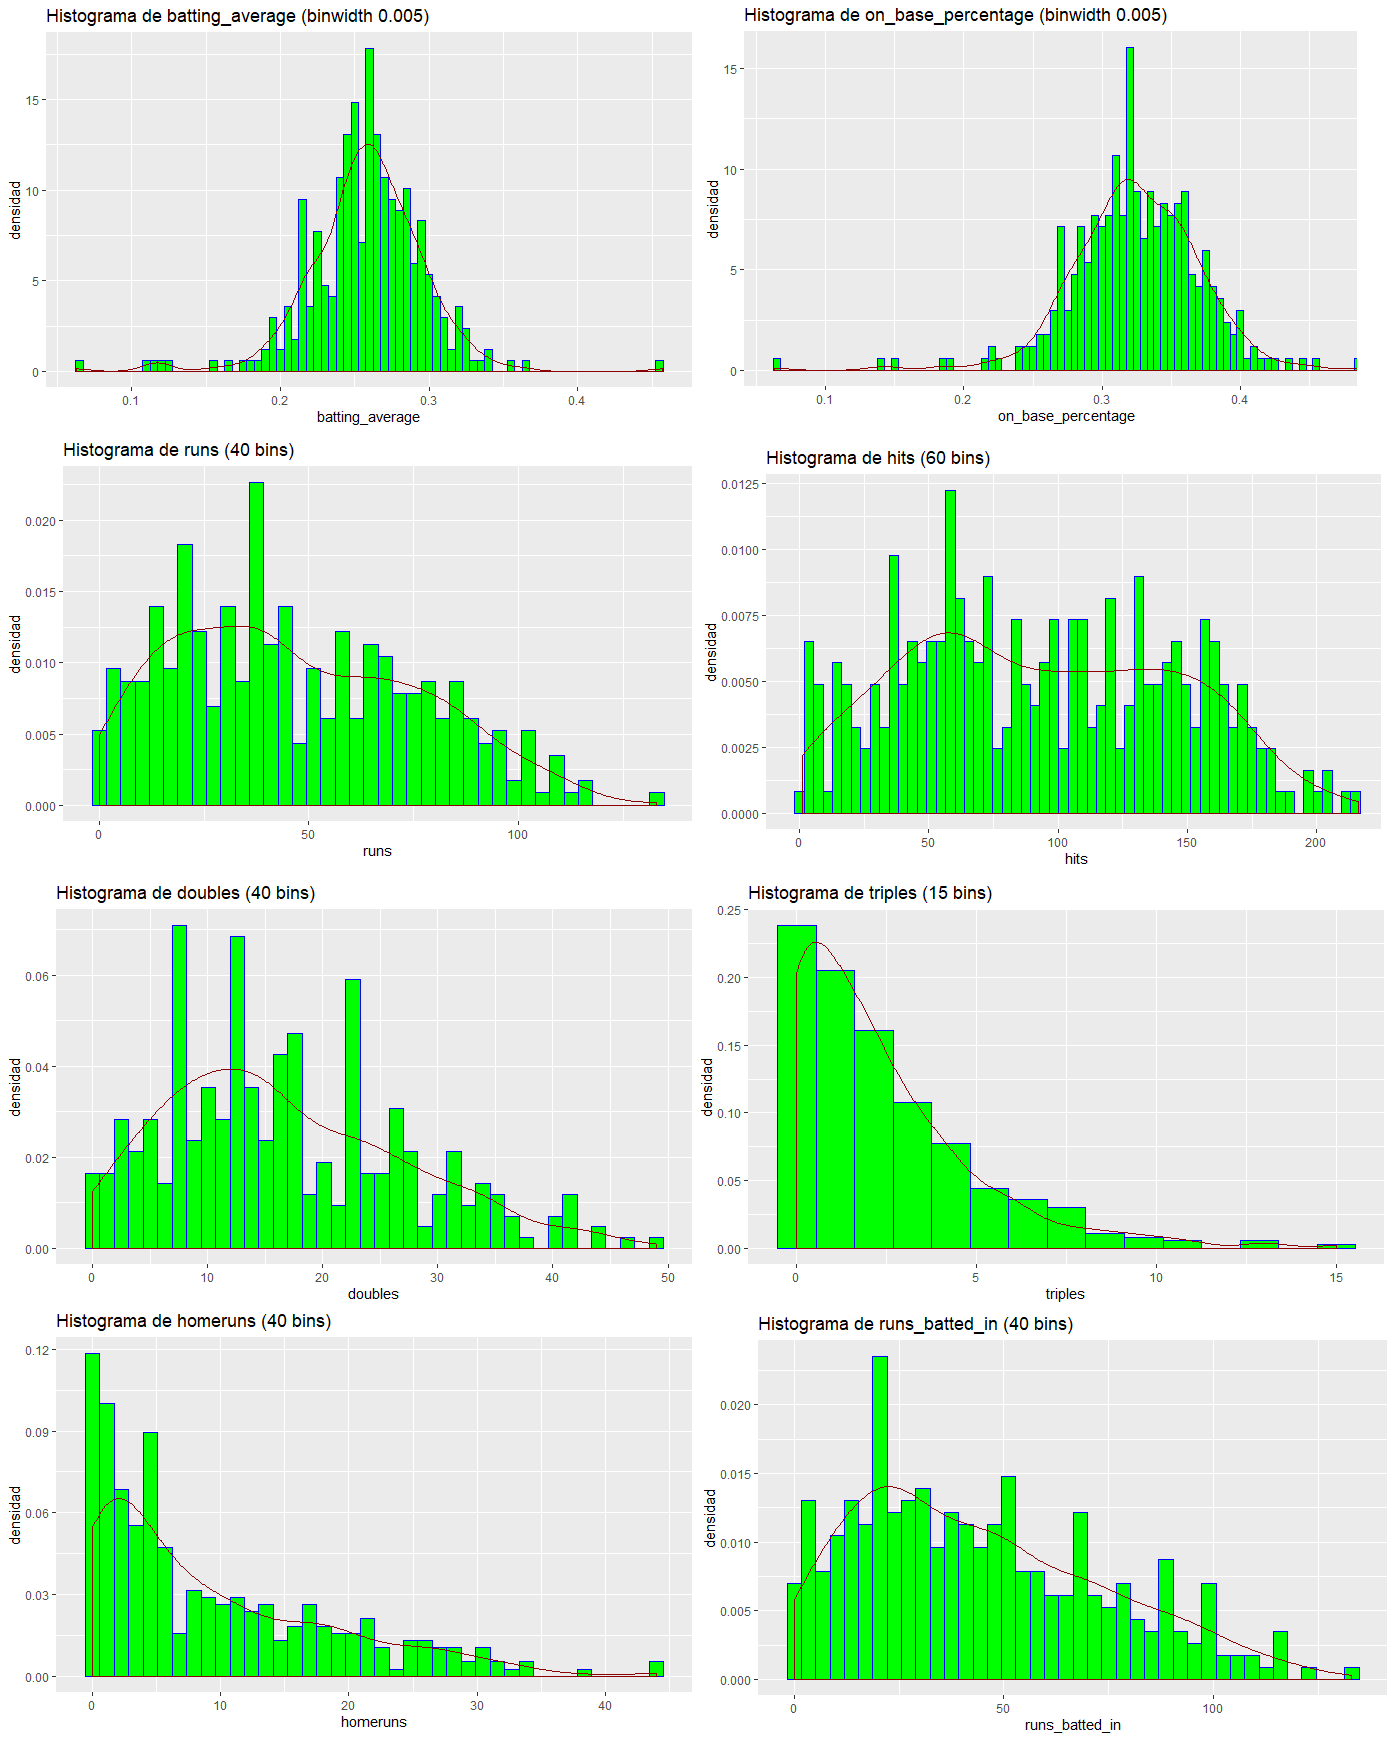
\includegraphics[scale=0.45]{images/histogram1.png}
\caption{Histogramas con estimación de curva de densidad para las 8 primeras variables numéricas (``baseball'').}
\end{figure}

\begin{figure}[H]
\centering
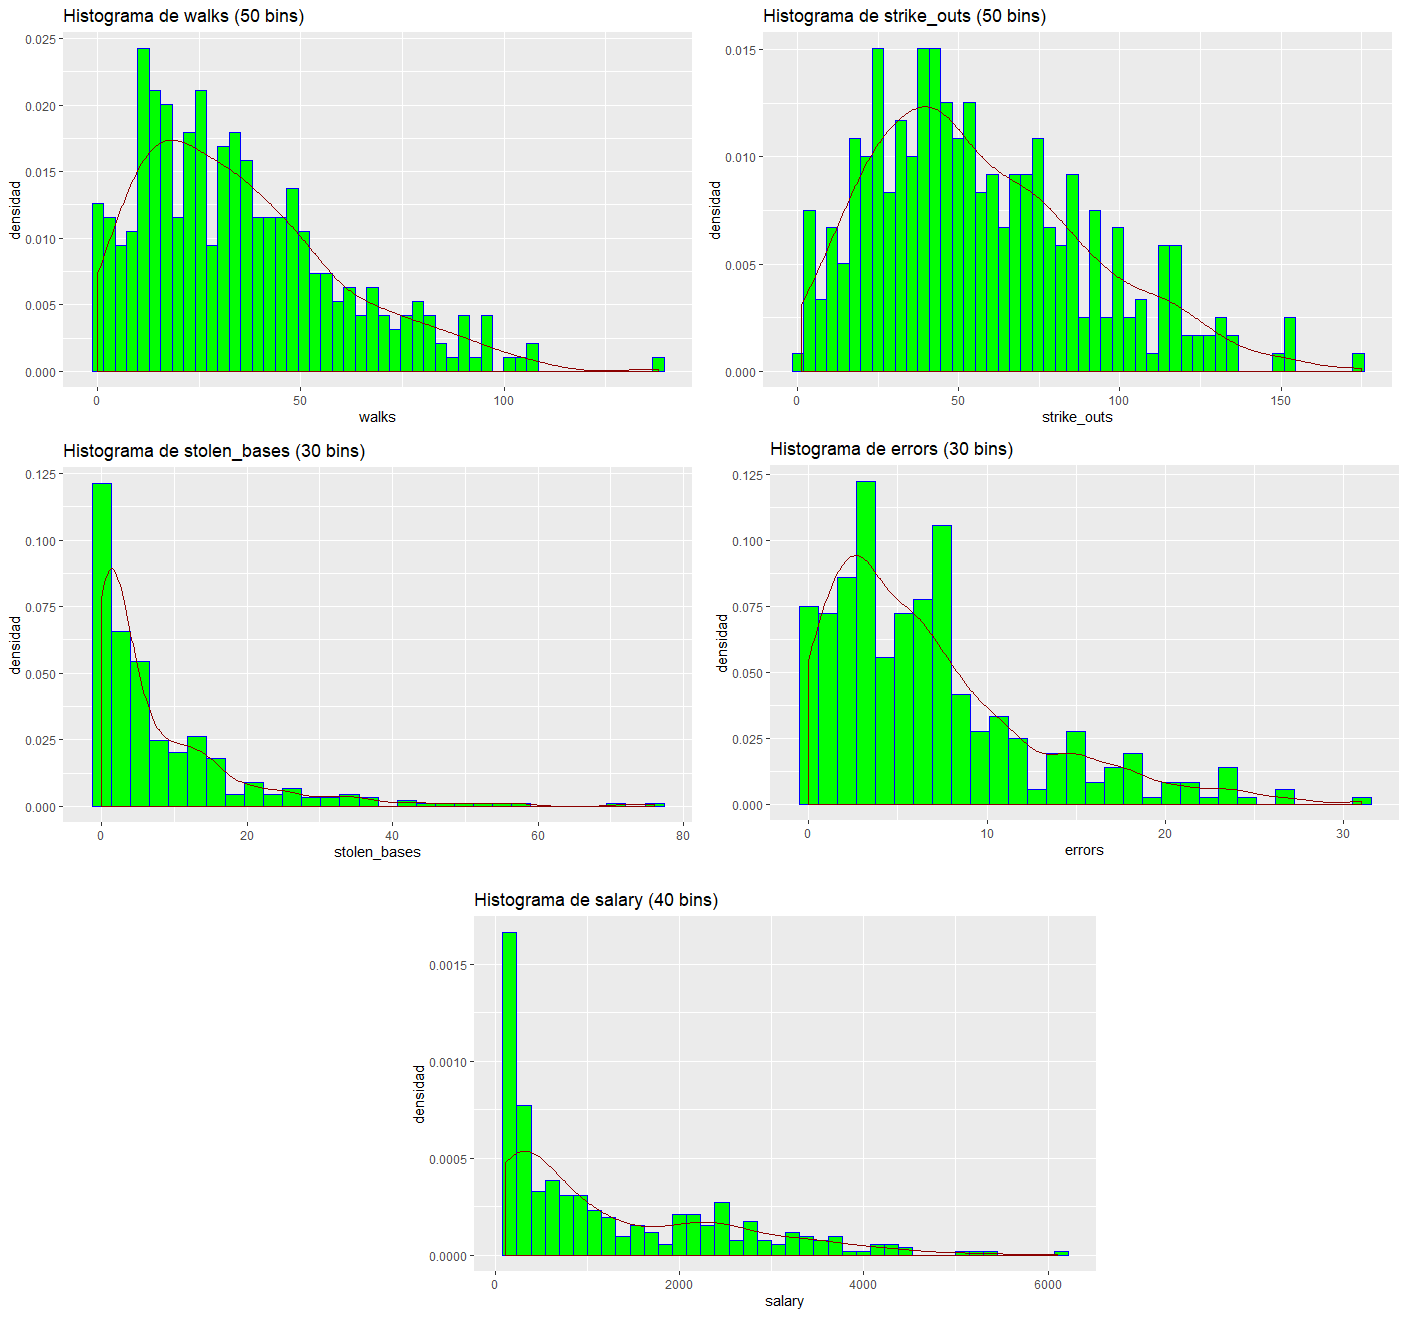
\includegraphics[scale=0.45]{images/histogram2.png}
\caption{Histogramas con estimación de curva de densidad para las 5 última variables numéricas (``baseball'').}
\end{figure}

En las dos primeras variables, observamos una distribución de los datos muy similar a la normal, con el centro de \textit(on\_base\_percentage) desplazado hacia la derecha y una cola un poco más larga a la izquierda (\textit{left-skewed}). \\

No obstante, la tendencia en la mayoría de las variables, es tener una cola prolongada hacia la derecha (\textit{right-skewed}). Esto es un indicativo de que tenemos muchas más muestras para los valores más bajos que para el resto de valores. Es algo lógico con respecto a la semántica de las variables. Son medidas de rendimiento en cantidades absolutas (también algunas medidas negativas), pero es razonable que el número de muestras sean más elevada para valores más bajos de las variables, porque puede ser tanto que un jugador ha jugado poco a lo largo de la temporada como que ha tenido un mal rendimiento. \\

Dentro de los estadísticos que tenemos hay alguno que podría tener una distribución multimodal, aunque la poca definición de las curvas y el conocimiento del significado de las variables hace que descarte tratarlas como tales. No obstante, el comportamiento de una de estas variables, \textit{hits}, es bastante peculiar. Si analizamos la definición del estadístico, en realidad es una interacción que suma los diferentes tipos de hits. He probado a crear una variable ``singles'' \textit{(hits - double - triples - homeruns)}.\\

Al generar esta nuestra variable aparece una muestra con un valor imposible (-12 singles). Es obvio que, a no ser que no hayamos comprendido algo sobre el problema, esa muestra tiene datos erróneos (tenemos 16 doubles y tan sólo 8 hits) Puesto que sólo es una, voy a eliminarla del dataset con el que trabajamos. Además, para garantizar que no es un error, he recurrido al enlace de las estadísticas de la MLB de esa temporada (https://www.baseball-reference.com/leagues/MLB/1991-batting-leaders.shtml) y he revisado si el top 10 de los ``singles'' de mi dataset se corresponden con los 10 que ofrece la página, cosa que ocurre. \\
	
Por otro lado, para ver las escalas y la situación general de los ``outliers'', vamos a utilizar un boxplot. He decidido sacar del mismo, la variable de salario, pues tiene una escala considerablemente distinta al resto de variables. \\

\begin{figure}[H]
\centering
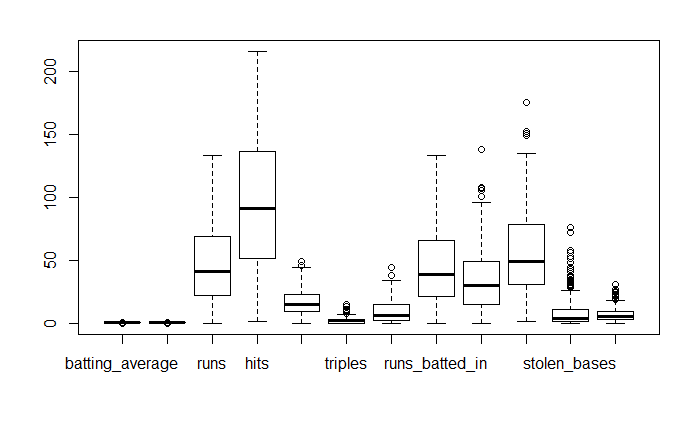
\includegraphics[scale=0.6]{images/boxplot.png}
\caption{Boxplot para las variables numéricas excepto el salario (``baseball'').}
\end{figure}


Aunque existen claras diferencias en escala, que nos dificultan determinar el rango de las variables que rondan el intervalo (0,1), este boxplot nos permite comprobar gráficamente que: las variables no tienen una escala propia para aplicar algoritmos como el k-nn para regresión y la abundancia de ``outliers'' en el dataset. \\


La siguiente representación gráfica (o más bien numérica) que vamos a utilizar es un correlograma (figura \ref{correplotbaseball}) entre los pares de variables numéricos. Puesto que no hemos asumido ninguna propiedad sobre todas las variables, vamos a utilizar el test de Kendall para calcular las correlaciones.\\

\begin{figure}[H]
\centering
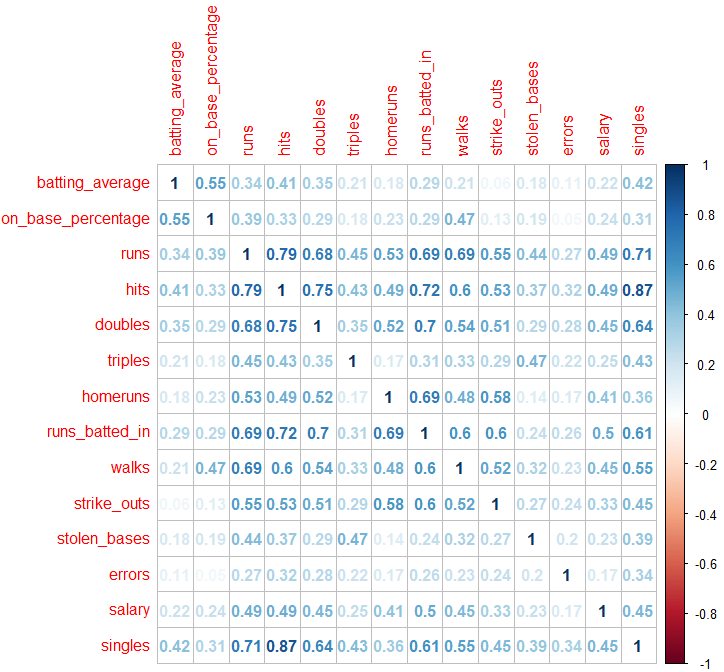
\includegraphics[scale=0.5]{images/corrplot_baseball.png}
\caption{Correlation-plot para las variables numéricas (``baseball'').}
\label{correplotbaseball}
\end{figure}


De la representación obtenida podemos observar que, además de la variable que nosotros hemos creado de forma intencional como combinación lineal de \textit{double, triples, homeruns y hits} todas las variables tienen un índice de correlación inferior a 0.8. El hecho de que exista una correlación tan fuerte entre \textit{hits} y \textit{singles} se debe a que la mayor parte de los \textit{hits} suelen ser de ese tipo. La segunda correlación más fuerte que encontramos la vemos entre \textit{hits y runs}, ya que toda carrera anotada va a tener un hit. No obstante, no es una correlación más fuerte porque también pueden existir \textit{hits} que no den lugar a anotar una carrera.

\subsection{Comprobación de hipótesis.}
\textbf{El \textit{``homerun''} es una de las jugadas más conocidas del béisbol, ¿está fuertemente relacionado de forma positiva con el salario?}\\

Para comprobarlo, vamos a crear un \textit{scatterplot} entre el número de \textit{homeruns} y el salario obtenido.\\

\begin{figure}[H]
\centering
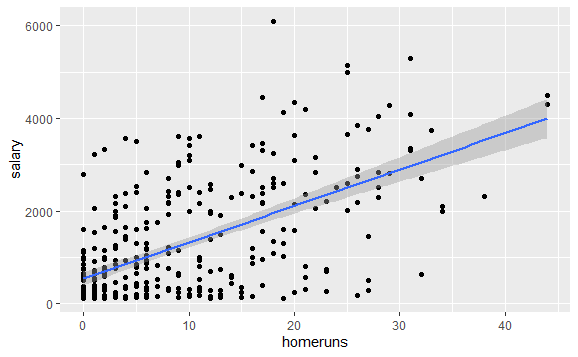
\includegraphics[scale=0.7]{images/homerun_salary.png}
\caption{Diagrama de dispersión entre el número de \textit{homeruns} y el salario con estimador lineal superpuesto.}
\label{homerunsalary}
\end{figure}

En rasgos generales, podríamos decir que conforme aumente el número de homeruns es más probable que el jugador obtenga un mejor salario. Sin embargo, parece que eso no siempre es el caso. En primer lugar, para cada valor de \textit{homeruns} existe una alta variabilidad en el rango de salarios obtenidos, es decir, si el valor de \textit{homeruns} influye en el salario hay otros factores que son más relevantes para determinarlo. En los extremos más bajos de ambas variables, existe un cúmulo considerable de muestras. Tanto vemos, la variabilidad de los salarios de los jugadores que no anotaron un \textit{homerun} en toda la temporada, como podemos observar que hasta 26-27 \textit{homeruns}, encontramos jugadores con salarios cercanos al mínimo registrado en el \textit{dataset}.\\

\textbf{Dentro de los estadísticos de béisbol que disponemos, tenemos dos de carácter negativo, \textit{strike-outs} para el bateador y \textit{errors} para un jugador defensivo, ¿implica ésto una disminución del salario de los jugadores?}\\

De nuevo, volvemos a usar \textit{scatterplots} para cada par de variables.

\begin{figure}[H]
\centering
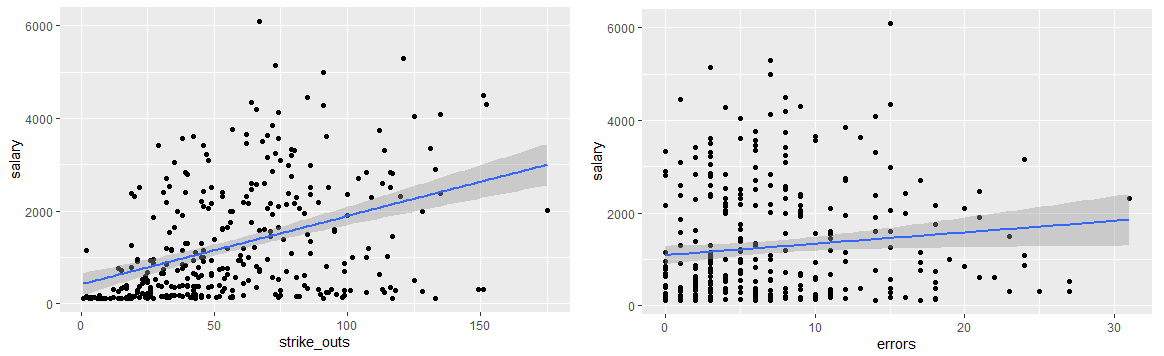
\includegraphics[scale=0.5]{images/strikeouts_errors.png}
\caption{Diagrama de dispersión entre el número de \textit{strike-outs}, número de errores y el salario con estimador lineal superpuesto.}
\label{homerunsalary}
\end{figure}

Resultan sorprendentes los resultados pues en ninguno de los casos podemos afirmar que un mal rendimiento del jugador implique un descenso en el salario. De hecho, en el caso del número de \textit{strike-outs} observamos que la tendencia general es que, a mayor número de fallos mejor salario se obtiene. Para poder comprender esta situación, hemos de tener en cuenta que es un estadístico absoluto por lo que los jugadores que más partidos jueguen podrán llegar a cometer más \textit{strike-outs} y existe una alta concentración de jugadores con un número de \textit{strike-outs} bajos en los umbrales inferiores de salario, quizás porque hayan jugado pocos partidos. En el caso de los errores, aunque podríamos ver una tendencia negativa si nos fijamos en la muestras que ocupan el centro del diagrama, al tener en cuenta el conjunto de todas las muestras parece ser que el número de errores es una variable bastante irrelevante a la hora de determinar el salario. \\

\textbf{En la MLB existen métodos como la arbitración que permiten a un jugador reclamar derechos sobre su salario, ¿está el salario acotado inferior y/o superiormente?}\\

Como podíamos observar tanto en los \textit{scatterplots} previos, como el histograma del salario que vemos de nuevo a continuación, existe una concentración inusualmente grande de valores cerca del valor mínimo registrado. \\

\begin{figure}[H]
\centering
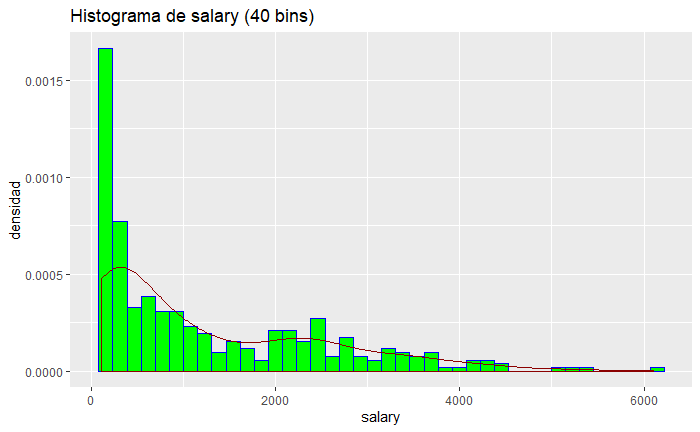
\includegraphics[scale=0.7]{images/salary.png}
\caption{Histograma del salario de los jugadores en la temporada con estimación de densidad superpuesta.}
\label{homerunsalary}
\end{figure}

Indagando por Internet, podemos confirmar que, efectivamente, existe un salario y mínimo, y en la temporada 1991/1992 era de 109000 dólares (que coincide con los 109 que nos salían de mínimo al analizar los datos en la tabla, los salarios están en miles de dólares en el \textit{dataset}). El salario no está acotado superiormente por un máximo.\\




\textbf{Ser agente libre (más de 6 años en la MLB a no ser que se finalice el contrato con el equipo) y disponer de arbitración (entre 3 y 6 años en la MLB), no sólo son mecanismos para mejorar la competitividad del salario de los jugadores, también son indicativos de la veteranía del jugador. ¿Tienen un salario mayor los jugadores con acceso a estos mecanismos?}\\

Vamos a ver qué ocurre con los salarios de los jugadores si tienen acceso al mecanismo de arbitración y si tienen acceso a ser agentes libres (hemos de tener en cuenta que, en este último caso, va a estar presente el ruido de ser agente libre porque el equipo finaliza el contrato con el jugador). Para ver la distribución de los salarios en ambos casos, utilizamos boxplots.

\begin{figure}[H]
\centering
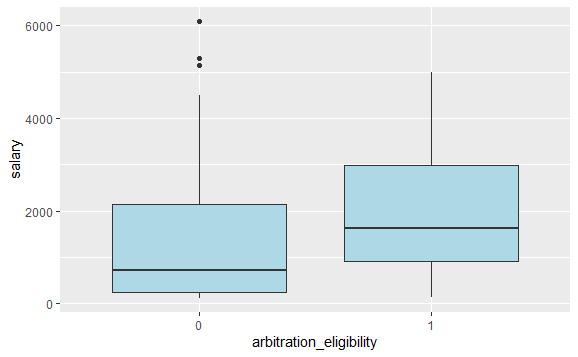
\includegraphics[scale=0.7]{images/arbitration_salary.png}
\caption{Boxplot del salario en función de la opción de solicitar arbitración (1=Sí).}
\label{boxplotarbitration}
\end{figure}

\begin{figure}[H]
\centering
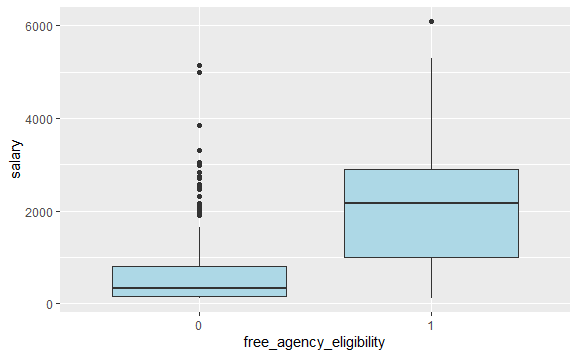
\includegraphics[scale=0.7]{images/agency_salary.png}
\caption{Boxplot del salario en función de la opción de ser agente libre (1=Sí).}
\label{boxplotarbitration}
\end{figure}

Podemos confirmar que, efectivamente, tener acceso a uno de estos mecanismos de competitividad/indicadores de veteranía ayuda a obtener un mejor salario. En los casos en los que se tiene acceso a ellos, tanto la media como el rango intercuartílico mejora, aunque siguen existiendo casos que siguen cobrando el salario mínimo.

\subsection{Descripción del conjunto de datos a partir de los apartados anteriores.}

En definitiva, el conjunto de datos nos proporciona datos sobre los salarios de los jugadores (en miles de dólares), estadísticos de rendimiento del jugador (la mayoría en medidas absolutas) y acceso a mecanismos de competitividad. Este \textit{dataset} parece contar la historia de cómo un gran número de jugadores de béisbol (quizás principiantes o no) reciben un salario muy bajo independientemente del rendimiento obtenido y la existencia de mecanismos (arbitración, ser agente libre, salario mínimo) que intentan defender los derechos del jugador como empleado del equipo.\\

En el dataset, hemos encontrado una abundancia de \textit{outliers}, muchos de ellos podrían ser de carácter natural pero al generar la única variable que hemos añadido, ``singles'', hemos detectado una muestra cuyos datos no tenían sentido y la hemos eliminado.

\newpage
\section{EDA - dataset de clasificación ``contraceptive''.}
\subsection{Descripción del dataset.}
El dataset \textit{``contraceptive''} contiene información recogida en una encuesta en Indonesia del año 1987 acerca del uso de método anticonceptivos por parte de mujeres casadas. El objetivo es determinar qué tipo de métodos anticonceptivos se utilizan (ninguna, método a corto plazo, método a largo plazo) basándonos en información demográfica y socioeconómica.
\subsection{Descripción del tipo de dato de entrada.}
Tras leer los datos, obtenemos un \textit{``data.frame''} con 1473 muestras y 10 atributos. Todos los valores del \textit{``data.frame''} tienen valores de tipo \textit{``integer''}. Gran parte de los datos son categorías, por lo que vamos a pasarlas a \textit{``factor''}. Las variables de las que disponemos son las siguientes:

\begin{itemize}
	\item \textbf{wife\_age} - Edad de la esposa. Es un valor numérico discreto (entero).
    \item \textbf{wife\_education} - Nivel de educación de la esposa en 4 niveles del 1 (bajo) al 4 (alto). Lo convertimos a \textit{``factor''}.
    \item \textbf{husband\_education} - Similar al anterior para el esposo. Lo convertimos a \textit{``factor''}.
    \item \textbf{children} - Número de hijos. Es un valor numérico discreto (entero).
    \item \textbf{wife\_religion} - Indica si la religión de la esposa es islámica. La convertimos a factor Sí (1) / No (0).
    \item \textbf{wife\_working} - Indica si la esposa tiene trabajo. La convertimos a factor Islámica (1) / No Islámica (0).
    \item \textbf{husband\_occupation} - Variable categórica que indica la ocupación del esposo entre 1 y 4. La convertimos a factor.
    \item \textbf{standard\_of\_living} - Nivel de vida entre 1 (bajo) y 4 (alto). La convertimos a factor.
    \item \textbf{media\_exposure} - Indica si han tenido acceso a algún medio de comunicación en el que han sido informados sobre métodos anticonceptivos. La convertimos a factor 0 (Buen acceso) / 1 (Mal acceso).
    \item \textbf{contraceptive\_method} - Indica si usa algún tipo de método anticonceptivo (1- No usa, 2- Usa un método efectivo a corto plazo, 3- Usa un método efectivo a largo plazo). Lo convertimos a factor.
\end{itemize}

Todas aquellas entre nivel 1 y 4 han sido transformadas a un factor ordenado(Bajo, Medio bajo, Medio alto, Alto).

\subsection{Cálculo de medidas de tendencia central, dispersión y dominio.}
Para las variables numéricas vamos a ver la media, la mediana y la moda, como medidas de tendencia central; la desviación típica y la desviación absoluta de la mediana, como medidas de dispersión; el mínimo y el máximo, para el dominio. En el caso de las variables categóricas, vamos a generar tablas de frecuencia absoluta de cada una de las clases.\\

\begin{longtable}{@{}c|rrrrrrr@{}}
\toprule
\textbf{Nombre} & \multicolumn{1}{c}{\textbf{Min}} & \multicolumn{1}{c}{\textbf{Max}} & \multicolumn{1}{c}{\textbf{Media}} & \multicolumn{1}{c}{\textbf{Mediana}} & \multicolumn{1}{c}{\textbf{Moda}}& \multicolumn{1}{c}{\textbf{\begin{tabular}[c]{@{}c@{}}Desviación \\ estándar\end{tabular}}} & \multicolumn{1}{c}{\textbf{\begin{tabular}[c]{@{}c@{}}Desviación \\ absoluta de la \\ mediana\end{tabular}}} \\* \midrule
\endhead
%
\textbf{wife\_age} & 16 & 49 & 32.5384 & 32 & 25 & 8.2272 & 8.8956 \\* \cmidrule(r){1-1}
\textbf{children} & 0 & 16 & 3.2614 & 3 & 1 & 2.3585 & 2.9652 \\* \bottomrule
\caption{Dominio, medidas de tendencia central y dispersión de las variables numéricas.}
\label{tab:tablamedidascontr}
\end{longtable}

\begin{table}[H]
\centering
\begin{tabular}{@{}ccccc@{}}
\toprule
\textbf{Variable} & \textbf{Bajo} & \textbf{Medio Bajo} & \textbf{Medio Alto} & \textbf{Alto} \\ \midrule
\textbf{\begin{tabular}[c]{@{}c@{}}wife\_education\\ (Educación de la esposa)\end{tabular}} & 152 & 334 & 410 & 577 \\
\textbf{\begin{tabular}[c]{@{}c@{}}husband\_education\\ (Educación del esposo)\end{tabular}} & 44 & 178 & 352 & 899 \\
\textbf{\begin{tabular}[c]{@{}c@{}}husband\_occupation\\ (Ocupación del esposo)\end{tabular}} & 436 & 425 & 585 & 27 \\
\textbf{\begin{tabular}[c]{@{}c@{}}standard\_of\_living\\ (Nivel de vida)\end{tabular}} & 129 & 229 & 431 & 684 \\ \cmidrule(r){1-3}
\textbf{Variable} & \textbf{No (0)} & \textbf{Sí (1)} &  &  \\ \cmidrule(r){1-3}
\textbf{\begin{tabular}[c]{@{}c@{}}wife\_religion\\ (¿Religión islámica?)\end{tabular}} & 220 & 1253 &  &  \\
\textbf{\begin{tabular}[c]{@{}c@{}}wife\_working\\ (¿Esposa trabajando?)\end{tabular}} & 369 & 1104 &  &  \\
\textbf{\begin{tabular}[c]{@{}c@{}}media\_exposure\\ (¿Poca exposición a\\  medios de comunicación?)\end{tabular}} & 1364 & 109 &  &  \\ \cmidrule(r){1-4}
\textbf{Variable} & \textbf{No Usa} & \textbf{Corto Plazo} & \textbf{Largo Plazo} &  \\ \cmidrule(r){1-4}
\textbf{\begin{tabular}[c]{@{}c@{}}contraceptive\_method\\ (Método anticonceptivo)\end{tabular}} & 629 & 333 & 511 &  \\ \cmidrule(r){1-4}
\end{tabular}
\caption{Tabla resumen de variables categóricas.}
\label{tab:factorresumen}
\end{table}


La mayoría de las personas encuestadas tiene un hijo único y la mayoría de personas tienen 25 años. No obstante, al tener en cuenta la distribución completa de encuestados la media y la mediana alcanza valores muy similares con 32 años y 3 hijos. En la tabla resumen de categorías vemos que nos encontramos ante un problema de clasificación desbalanceado (hay muchas menos muestras de personas que usan métodos a corto plazo que las de a largo plazo o las que no usan). También observamos cómo algunos de los valores para las categorías están representados por un subconjunto de muestras muy pequeño.

\subsection{Detección de \textit{missing values} y muestras duplicadas.}
No hemos detectado ninguna muestra con \textit{missing values} indicados con \textit{NA} así como los dominios de todas las muestras son razonables conforme a su significado. Hemos encontrado un total de 46 muestras duplicadas que van a ser eliminadas. Es importante eliminar estos casos ya que, si dejáramos las muestras repetidas en el \textit{dataset}, esa situación tendría el doble de relevancia que el resto de casos (si está repetida una vez, triple si está repetida dos veces, etc.). Una vez hemos eliminado esas muestras, vamos a actualizar las tablas previas para ver cómo se ajustan ahora las tendencias en nuestro \textit{dataset}.

\begin{longtable}{@{}c|rrrrrrr@{}}
\toprule
\textbf{Nombre} & \multicolumn{1}{c}{\textbf{Min}} & \multicolumn{1}{c}{\textbf{Max}} & \multicolumn{1}{c}{\textbf{Media}} & \multicolumn{1}{c}{\textbf{Mediana}} & \multicolumn{1}{c}{\textbf{Moda}}& \multicolumn{1}{c}{\textbf{\begin{tabular}[c]{@{}c@{}}Desviación \\ estándar\end{tabular}}} & \multicolumn{1}{c}{\textbf{\begin{tabular}[c]{@{}c@{}}Desviación \\ absoluta de la \\ mediana\end{tabular}}} \\* \midrule
\endhead
%
\textbf{wife\_age} & 16 & 49 & 32.5046 & 32 & 25 & 8.2159 & 8.8956 \\* \cmidrule(r){1-1}
\textbf{children} & 0 & 16 & 3.2849 & 3 & 2 & 2.3777 & 2.9652 \\* \bottomrule
\caption{Dominio, medidas de tendencia central y dispersión tras eliminar duplicados. Dataset: ``contraceptive''}
\label{tab:tablamedidascontr2}\\
\end{longtable}

\begin{table}[H]
\centering
\begin{tabular}{@{}ccccc@{}}
\toprule
\textbf{Variable} & \textbf{Bajo} & \textbf{Medio Bajo} & \textbf{Medio Alto} & \textbf{Alto} \\ \midrule
\textbf{\begin{tabular}[c]{@{}c@{}}wife\_education\\ (Educación de la esposa)\end{tabular}} & 150 & 331 & 401 & 543 \\
\textbf{\begin{tabular}[c]{@{}c@{}}husband\_education\\ (Educación del esposo)\end{tabular}} & 44 & 176 & 347 & 858 \\
\textbf{\begin{tabular}[c]{@{}c@{}}husband\_occupation*\\ (Ocupación del esposo)\end{tabular}} & 436 & 425 & 585 & 27 \\
\textbf{\begin{tabular}[c]{@{}c@{}}standard\_of\_living\\ (Nivel de vida)\end{tabular}} & 129 & 229 & 431 & 684 \\ \cmidrule(r){1-3}
\textbf{Variable} & \textbf{No (0)} & \textbf{Sí (1)} &  &  \\ \cmidrule(r){1-3}
\textbf{\begin{tabular}[c]{@{}c@{}}wife\_religion\\ (¿Religión islámica?)\end{tabular}} & 215 & 1210 &  &  \\
\textbf{\begin{tabular}[c]{@{}c@{}}wife\_working\\ (¿Esposa trabajando?)\end{tabular}} & 360 & 1065 &  &  \\
\textbf{\begin{tabular}[c]{@{}c@{}}media\_exposure\\ (¿Poca exposición a\\  medios de comunicación?)\end{tabular}} & 1316 & 109 &  &  \\ \cmidrule(r){1-4}
\textbf{Variable} & \textbf{No Usa} & \textbf{Corto Plazo} & \textbf{Largo Plazo} &  \\ \cmidrule(r){1-4}
\textbf{\begin{tabular}[c]{@{}c@{}}contraceptive\_method\\ (Método anticonceptivo)\end{tabular}} & 614 & 316 & 495 &  \\ \cmidrule(r){1-4}
\end{tabular}
\caption{Tabla resumen de variables categóricas tras eliminar muestras duplicadas.}
\label{tab:factorresumen2}
\end{table}

Tras actualizar los datos vemos que, por regla general, las distribuciones se mantienen más o menos igual. El problema sigue siendo un problema de clasificación desbalanceado, ha habido clases en las que las muestras repetidas estaban concentradas en una de las clases (\textit{``media\_exposure''}, por ejemplo) y resulta curioso que la moda haya pasado de tener 1 hijo a tener 2. Esto último se debe, en gran parte a la concentración	de muestras que hay alrededor de esos valores y la poca diferencia entre ambos (tras eliminar muestras duplicadas, 266 con un hijo, 272 con 2 hijos).\\

\subsection{Gráficos que permitan visualizar los datos adecuadamente.}
En cuanto a gráficos univariables, vamos a utilizar histogramas con estimación de curva de densidad superpuesta para las dos variables numéricas, para las variables categóricas vamos a utilizar diagramas de barras y veremos la diferencia de escalas de las variables numéricas en un boxplot.
\begin{figure}[H]
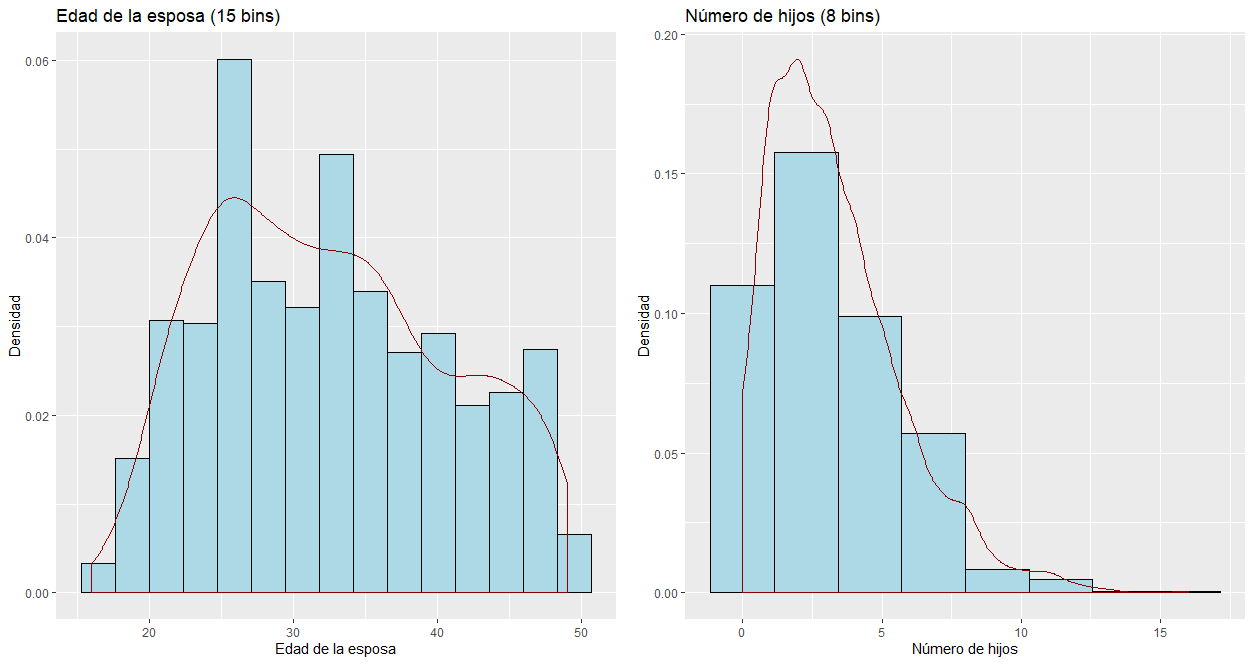
\includegraphics[scale=0.5]{images/contraceptive_histogram.png}
\caption{Histograma con estimación de curva de densidad superpuesta para variables numéricas.}
\end{figure}

En el caso de la edad de la esposa cuesta ver la posibilidad de normalidad en esa distribución gráfica, existen diferentes puntos de inflexión en la distribución pero ninguno lo suficientemente destacado como para plantear la posibilidad de una distribución multimodal, presenta una \textit{skewness} positiva muy ligera. En el caso del número de hijos, se podría apreciar normalidad realizando alguna transformación como la logarítmica, ya que resulta evidente el alto nivel de \textit{skewness} positiva que tiene la distribución con el cúmulo de muestras rondando los valores más bajos (entre 0 y 3). \\

\begin{figure}[H]
\centering
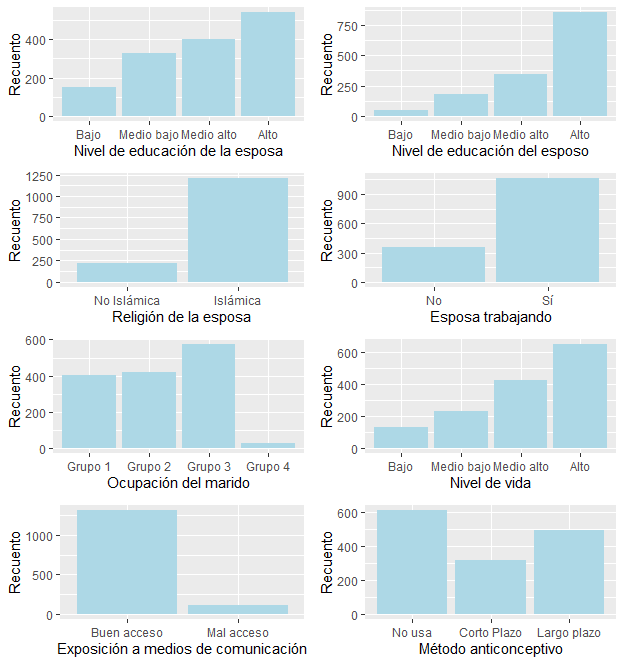
\includegraphics[scale=0.7]{images/barplot_contraceptive.png}
\caption{Diagramas de barras para las variables categóricas.}
\end{figure}

De este diagrama observamos que mientras que el nivel de educación de la esposa se encuentra bastante repartido en los distintos niveles, el nivel de educación del esposo es alto en un mayor número de casos, la mayoría de las mujeres son islámicas y tienen un trabajo en el momento de la encuesta, la mayoría tiene acceso a medios de comunicación y tenemos más gente en la encuesta que afirmar llevar un nivel de vida en los umbrales altos con respecto a las de los umbrales bajos.

\begin{figure}[H]
\centering
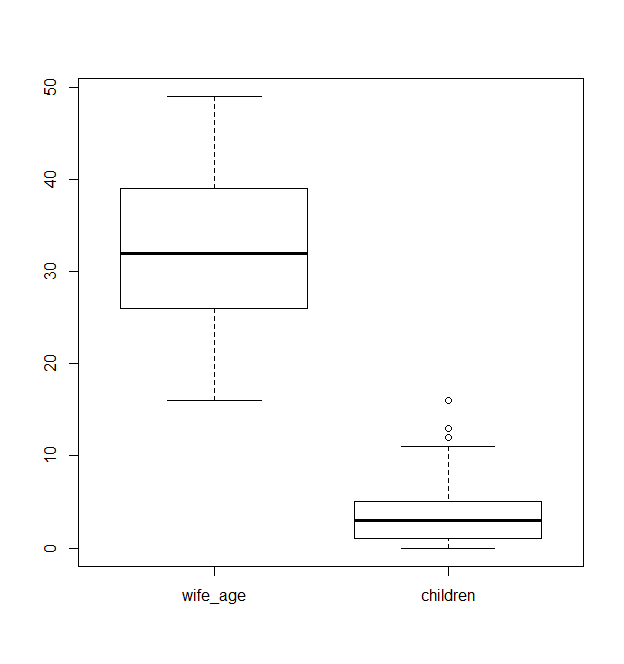
\includegraphics[scale=0.7]{images/boxplot_contraceptive.png}
\caption{Boxplot para las variables numéricas.}
\end{figure}
De este boxplot, vemos que no se detecta ningún \textit{``outlier''} univariable basando en rango intercuartílico para \textit{``wife\_age''} aunque sí se detectan algunos para \textit{``children''} en sus valores más altos. 

\newpage
\subsection{Planteamiento de hipótesis.}
\begin{itemize}
	\item ¿Existe desconocimiento sobre el uso de anticonceptivos? Es decir, ¿es más habitual que una persona que tiene acceso a medios de comunicación en los que pueda haberse informado acerca de ellos usa métodos anticonceptivos?
	\item ¿Son más habituales los métodos anticonceptivos a corto plazo en parejas jóvenes y los de largo plazo en parejas de edad madura?
	\item ¿Influye el número de hijos en el uso de métodos anticonceptivos?
\end{itemize}
\subsection{Comprobación de hipótesis.}

\textbf{¿Existe desconocimiento sobre el uso de anticonceptivos? Es decir, ¿es más habitual que una persona que tiene acceso a medios de comunicación en los que pueda haberse informado acerca de ellos usa métodos anticonceptivos?}\\

\begin{figure}[H]
\centering
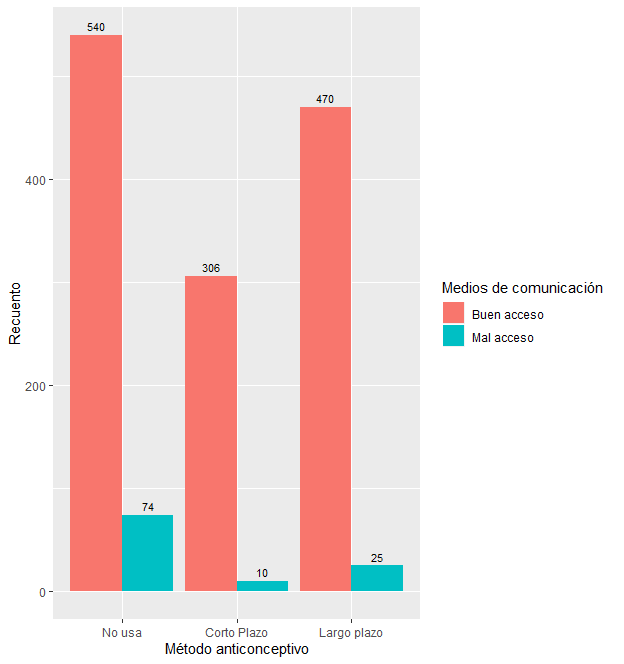
\includegraphics[scale=0.7]{images/hipo1.png}
\caption{Diagrama de barras para el uso de anticonceptivos en función de exposición a medios.}
\end{figure}

Como ya sabíamos, existe un número de personas que tienen mal acceso (109) muy inferior al de las personas que buen acceso (1316). No obstante, vemos que 74 de los 109 no usan métodos anticonceptivos (67,89 \%), mientras que los informados a través de los medios de comunicación 540 de los 1316 no usan métodos anticonceptivos (41,03 \%), así que parece ser que ese acceso a la información es bastante relevante.\\

\textbf{¿Son más habituales los métodos anticonceptivos a corto plazo en parejas jóvenes y los de largo plazo en parejas de edad madura?}\\
\begin{figure}[H]
\centering
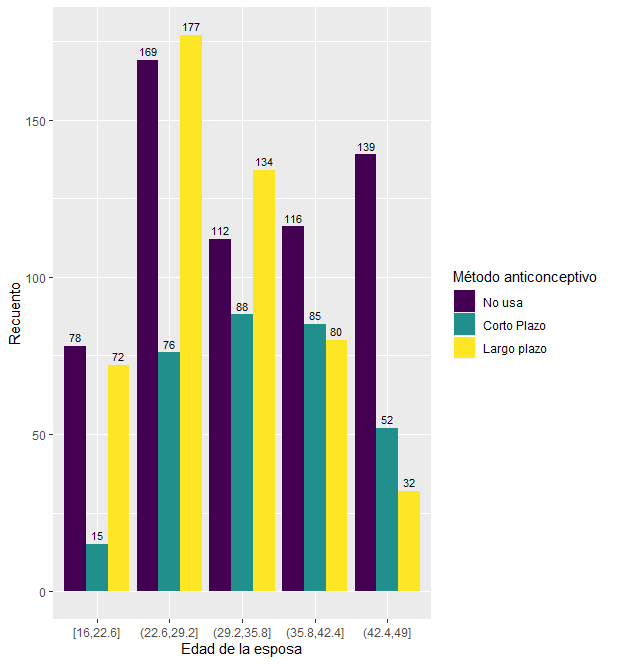
\includegraphics[scale=0.7]{images/hipo2.png}
\caption{Diagrama de barras para el uso de anticonceptivos en función de la edad de la esposa.}
\end{figure}

De la gráfica podemos observar que este hipótesis no es cierta. En esta gráfica, hemos dividido las edades de la esposas en 5 intervalos. En el subgrupo de mujeres más jóvenes vemos cómo lo más frecuente es no usar métodos anticonceptivos, seguido de cerca del uso de métodos anticonceptivos a largo plazo y con muy pocos casos de usos de métodos anticonceptivos a corto plazo. Por otro lado, conforme vamos llegando a las mujeres de edad más madura encontramos un menor número de métodos anticonceptivos a largo plazo. Por tanto, la tendencia general de nuestra población es la de no usar métodos anticonceptivos aunque entre los grupos más jóvenes es habitual usar métodos anticonceptivos, existiendo una preferencia del uso de métodos a largo plazo con respecto a los métodos de corto plazo.\\

\textbf{¿Influye el número de hijos en el uso de métodos anticonceptivos?}\\

Para ello, vamos a discretizar nuestra variable número de hijos acorde al siguiente criterio y la vamos a meter en la variable \textit{``children.cat''}.

\begin{itemize}
	\item Sin hijos. Tiene 0 hijos.
	\item Hijo único. Tiene 1 hijo.
	\item Algunos hijos. Esta valor cubre el hecho de tener un número de hijos habitual (2-3). No incluyo el valor 1 para que de alguna manera este valor cubra las implicaciones que pueda tener el hecho de que los hijos tengan hermanos.
	\item Muchos hijos. 4 hijos o más.
\end{itemize}

\begin{figure}[H]
\centering
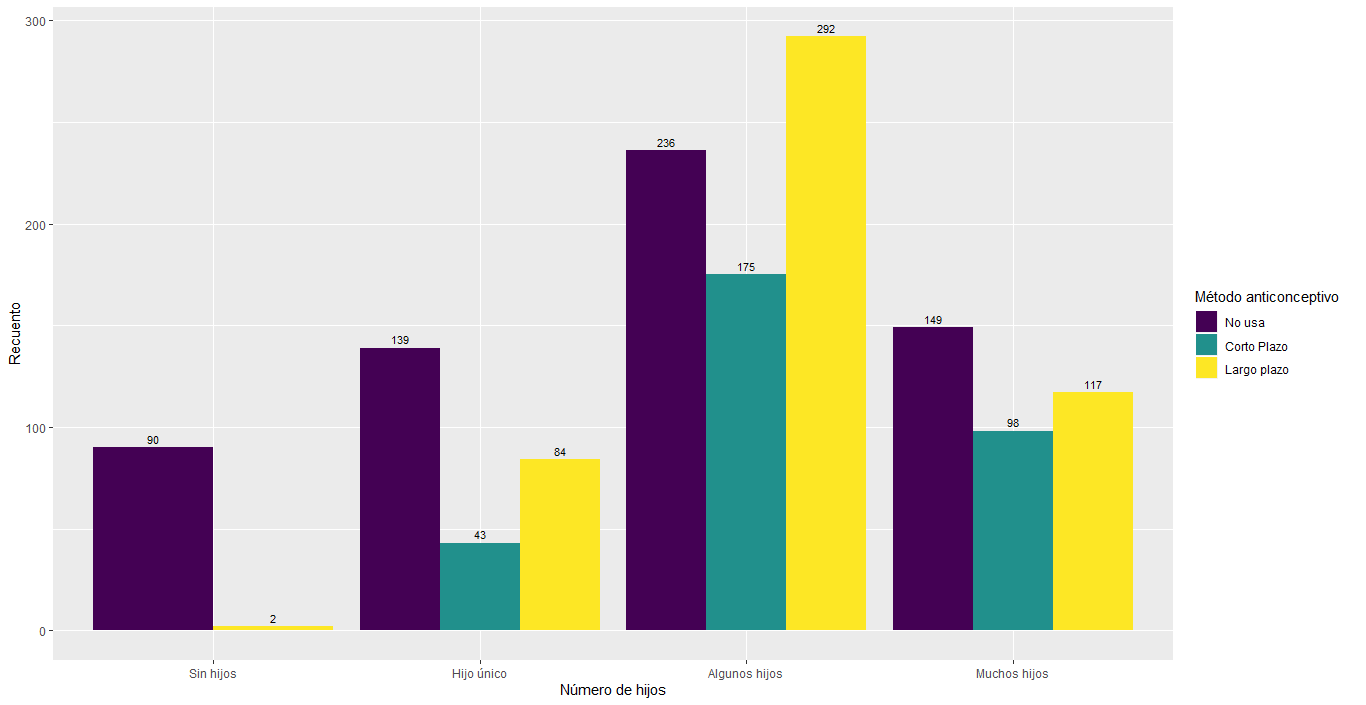
\includegraphics[scale=0.5]{images/hipo3.png}
\caption{Diagrama de barras para el uso de anticonceptivos en función del número de hijos.}
\end{figure}

Lo primero que observamos es que la gran mayoría de parejas sin hijos no utilizan ningún método anticonceptivo. Cuando tienen un único hijo 
hay casi el mismo número de personas que utilizan métodos anticonceptivos (127) con respecto a los 139 que no usan, aunque prefieren el uso de métodos anticonceptivos a largo plazo. Cuando se tienen 2 o 3 hijos, nos encontramos con el caso en el que es mucho más habitual el uso de métodos anticonceptivos (467) frente a los 236 que no usan anticonceptivos (casi la mitad). Cuando se tienen muchos hijos, sigue siendo más habitual el uso de métodos anticonceptivos (215) frente a los 149 que no usan anticonceptivos.

\subsection{Descripción del conjunto de datos a partir de los apartados anteriores.}
El conjunto de datos con el que trabajamos nos da información acerca del uso de métodos anticonceptivos en Indonesia en 1982. El problema de clasificación a resolver consiste en determinar qué tipo de método anticonceptivo se utiliza (ninguno, a corto plazo o a largo plazo) y dicho problema tienen las clases desbalanceadas. La mayor parte de los datos con los trabajamos son variables categóricas y hacen referencia al nivel de educación de la pareja, el trabajo, su religión o el nivel de vida. Además, tenemos dos variables continuas, la edad de la mujer y el número de hijos. Para el número de hijos, vamos a considerar la categorización usada en la última hipótesis propuesta. De las hipótesis hemos deducido que:

\begin{itemize}
	\item Es más probable que una persona que ha sido informada a través de los medios de comunicación de métodos anticonceptivos haga un mayor uso de ellos.
	\item La edad de las mujeres influye en el uso de métodos anticonceptivos. En las mujeres más jóvenes es habitual tanto no usar métodos anticonceptivos como métodos anticonceptivos a largo plazo. En las mujeres de edad más madura es mucho más habitual no usar anticonceptivos y en mujeres de edad media es más habitual usar algún método anticonceptivo, existiendo una tendencia general a utilizar métodos anticonceptivos a largo plazo.
	\item El número de hijos influye en el uso de métodos anticonceptivos. Si no se tienen hijos, es habitual que no se usen métodos anticonceptivos. Cuando se tiene un único hijo, hay mucha gente que sigue sin usar anticonceptivos pero aparece un grupo de personas de un tamaño similar que si utiliza métodos anticonceptivos. Cuando se tienen entre 2 o más hijos, lo habitual es usar algún tipo de anticonceptivo.
\end{itemize}

\newpage
\chapter{Regresión.}
De la parte del análisis exploratorio de datos, hemos realizados dos modificaciones sobre el \textit{dataset}. Una de ellas es añadir una nueva variable \textit{``singles''}, pues tenemos una variable \textit{``hits''} que es la suma de los \textit{``singles'', ``doubles'', ``triples'' y ``homeruns''} del jugador. Puesto que la mayoría de \textit{``hits''} son \textit{``singles''} están altamente correlados. En esta sección determinaremos con cuál quedarnos, si es que nos quedamos con alguno. 
Además, hemos detectado una muestra con datos incorrectos (tenía más \textit{``doubles''} que \textit{``hits''}). Esa muestra será eliminada de las particiones en las que se encuentre presente.

\section[Regresión lineal simple]{Utilizar el modelo de regresión lineal simple sobre cada regresor (variable de entrada) para obtener los modelos correspondientes. Si el dataset incluye más de 5 regresores, seleccione de manera justificada los 5 que considere más relevantes. Una vez obtenidos los modelos, elegir el que considere más adecuado para su conjunto de datos según las medidas de calidad conocidas.}
El \textit{dataset} con el que trabajo tiene más de 5 variables, así que \textbf{voy a tomar las 5 variables que se encuentran más correladas con la variable objetivo} (\textit{salary}). Para ello, voy a recurrir al gráfico de correlaciones planteado en la figura \ref{correplotbaseball} de la parte del análisis exploratorio de datos. Puesto que no hemos asegurado ninguna propiedad de los datos, hemos usado el test de Kendall para calcular las correlaciones.\\

En la imagen, sólo se ven los dos primeros decimales. Al inicio del script de R para regresión, se calcula de nuevo la correlación y se seleccionan las 5 más correladas teniendo en cuenta todos los decimales, que son:\\

\begin{itemize}
	\item \textbf{runs\_batted\_in} Correlación 0.5011 con \textit{salary}. [fit1]
	\item \textbf{runs} Correlación 0.4936 con \textit{salary}. [fit2]
	\item \textbf{hits} Correlación 0.4902 con \textit{salary}. [fit3]
	\item \textbf{doubles} Correlación 0.4553 con \textit{salary}. [fit4]
	\item \textbf{singles} Correlación 0.4501 con \textit{salary}. [fit5]
\end{itemize}

La \textbf{metodología} para realizar este apartado va a ser generar los modelos y ver su valores de R cuadrado ajustado para ver el que mejor explica teóricamente el conjunto completo. No obstante, para determinar cuál es el mejor vamos a coger el que tenga menor error cuadrático medio en los 5 \textit{folds} propuestos con el \textit{dataset}. Las variable usada consta en el pie de cada tabla.

\begin{table}[H]
\footnotesize
\centering
\begin{tabular}{cccccc}
\hline
\textbf{Modelo} & \multicolumn{5}{c}{\textbf{Residuos}} \\ \hline
\textit{\textbf{fit1}} & \textbf{Min} & \textbf{1Q} & \textbf{Mediana} & \textbf{3Q} & \textbf{Max} \\ \cline{2-6} 
\multicolumn{1}{l}{} & -2587.3 & -511.3 & -65.3 & 454.8 & 3281.7 \\ \cline{1-5}
\textbf{Coeficiente} & \textbf{Estimación} & \textbf{Std. Error} & \textbf{t value} & \textbf{PR(\textgreater{}|t|)} & \multicolumn{1}{l}{} \\ \cline{1-5}
(Intercept) & 14.078 & 90.881 & 0.155 & 0.877 &  \\
runs\_batted\_in & 28.042 & 1.712 & 16.378 & \textless{}2e-16 & *** \\ \cline{1-5}
\textbf{Res Std Error} & \textbf{Mult R-squared} & \textbf{Adj R-squared} & \textbf{F-statistic} & \textbf{p-value} & \multicolumn{1}{l}{} \\ \cline{1-5}
925.1; 334 df & 0.4454 & \textbf{0.4437} & 268.2; 1; 334 df & \textless{}2.2e-16 & \multicolumn{1}{l}{} \\ \hline
\textbf{MSE Fold 1} & \textbf{MSE Fold 2} & \textbf{MSE Fold 3} & \textbf{MSE Fold 4} & \textbf{MSE Fold 5} & \multicolumn{1}{l}{\textbf{Media MSE}} \\ \hline
683762 & 781996.1 & 985608.7 & 985634.9 & 856974.5 & \textbf{858795.2}
\end{tabular}
\caption{Regresión lineal simple: salary $\sim$ runs\_batted\_in. {[}fit1{]}}
\label{tab:fit1}
\end{table}

\begin{table}[H]
\footnotesize
\centering
\begin{tabular}{cccccc}
\hline
\textbf{Modelo} & \multicolumn{5}{c}{\textbf{Residuos}} \\ \hline
\textit{\textbf{fit2}} & \textbf{Min} & \textbf{1Q} & \textbf{Mediana} & \textbf{3Q} & \textbf{Max} \\ \cline{2-6} 
\multicolumn{1}{l}{} & -2217 & -572.9 & -54.6 & 432 & 3318.2 \\ \cline{1-5}
\textbf{Coeficiente} & \textbf{Estimación} & \textbf{Std. Error} & \textbf{t value} & \textbf{PR(\textgreater{}|t|)} & \multicolumn{1}{l}{} \\ \cline{1-5}
(Intercept) & -36.182 & 97.889 & -0.37 & 0.712 &  \\
runs & 27.627 & 1.783 & 15.49 & \textless{}2e-16 & *** \\ \cline{1-5}
\textbf{Res Std Error} & \textbf{Mult R-squared} & \textbf{Adj R-squared} & \textbf{F-statistic} & \textbf{p-value} & \multicolumn{1}{l}{} \\ \cline{1-5}
947.5; 334 df & 0.4182 & \textbf{0.4165} & 240.1; 1; 334 df & \textless{}2.2e-16 & \multicolumn{1}{l}{} \\ \hline
\textbf{MSE Fold 1} & \textbf{MSE Fold 2} & \textbf{MSE Fold 3} & \textbf{MSE Fold 4} & \textbf{MSE Fold 5} & \multicolumn{1}{l}{\textbf{Media MSE}} \\ \hline
808383.9 & 807984.2 &1027011.0 & 886622.0 &1020250.4 & \textbf{910050.3}
\end{tabular}
\caption{Regresión lineal simple: salary $\sim$ runs. {[}fit2{]}}
\label{tab:fit2}
\end{table}

\begin{table}[H]
\footnotesize
\centering
\begin{tabular}{cccccc}
\hline
\textbf{Modelo} & \multicolumn{5}{c}{\textbf{Residuos}} \\ \hline
\textit{\textbf{fit3}} & \textbf{Min} & \textbf{1Q} & \textbf{Mediana} & \textbf{3Q} & \textbf{Max} \\ \cline{2-6} 
\multicolumn{1}{l}{} & -2151.8 & -560.7 & -68.3 & 377.3 & 3646.1 \\ \cline{1-5}
\textbf{Coeficiente} & \textbf{Estimación} & \textbf{Std. Error} & \textbf{t value} & \textbf{PR(\textgreater{}|t|)} & \multicolumn{1}{l}{} \\ \cline{1-5}
(Intercept) & -130.902 & 109.521 & -1.195 & 0.233 &  \\
hits & 14.855 & 1.029 & 14.442 & \textless{}2e-16 & *** \\ \cline{1-5}
\textbf{Res Std Error} & \textbf{Mult R-squared} & \textbf{Adj R-squared} & \textbf{F-statistic} & \textbf{p-value} & \multicolumn{1}{l}{} \\ \cline{1-5}
974.6; 334 df & 0.3844 & \textbf{0.3826} & 208.6; 1; 334 df & \textless{}2.2e-16 & \multicolumn{1}{l}{} \\ \hline
\textbf{MSE Fold 1} & \textbf{MSE Fold 2} & \textbf{MSE Fold 3} & \textbf{MSE Fold 4} & \textbf{MSE Fold 5} & \multicolumn{1}{l}{\textbf{Media MSE}} \\ \hline
894572.4 & 850238.5 & 1120561.7 & 956445.6 & 956971.2 & \textbf{955757.9}
\end{tabular}
\caption{Regresión lineal simple: salary $\sim$ hits. {[}fit3{]}}
\label{tab:fit3}
\end{table}

\begin{table}[H]
\footnotesize
\centering
\begin{tabular}{cccccc}
\hline
\textbf{Modelo} & \multicolumn{5}{c}{\textbf{Residuos}} \\ \hline
\textit{\textbf{fit4}} & \textbf{Min} & \textbf{1Q} & \textbf{Mediana} & \textbf{3Q} & \textbf{Max} \\ \cline{2-6} 
\multicolumn{1}{l}{} & -2534.3 & -521.8 & -165.6 & 386.0 & 3122.5 \\ \cline{1-5}
\textbf{Coeficiente} & \textbf{Estimación} & \textbf{Std. Error} & \textbf{t value} & \textbf{PR(\textgreater{}|t|)} & \multicolumn{1}{l}{} \\ \cline{1-5}
(Intercept) & 109.898 & 104.126 & 1.055 & 0.292 &  \\
doubles & 68.485 & 5.291 & 12.944 & \textless{}2e-16 & *** \\ \cline{1-5}
\textbf{Res Std Error} & \textbf{Mult R-squared} & \textbf{Adj R-squared} & \textbf{F-statistic} & \textbf{p-value} & \multicolumn{1}{l}{} \\ \cline{1-5}
1014; 334 df & 0.3341 & \textbf{0.3321} & 167.5; 1; 334 df & \textless{}2.2e-16 & \multicolumn{1}{l}{} \\ \hline
\textbf{MSE Fold 1} & \textbf{MSE Fold 2} & \textbf{MSE Fold 3} & \textbf{MSE Fold 4} & \textbf{MSE Fold 5} & \multicolumn{1}{l}{\textbf{Media MSE}} \\ \hline
818589.5 & 886488.3 & 1350084.4 & 1116089.0 & 988923.8 & \textbf{1032035}
\end{tabular}
\caption{Regresión lineal simple: salary $\sim$ doubles. {[}fit4{]}}
\label{tab:fit4}
\end{table}

\begin{table}[H]
\footnotesize
\centering
\begin{tabular}{cccccc}
\hline
\textbf{Modelo} & \multicolumn{5}{c}{\textbf{Residuos}} \\ \hline
\textit{\textbf{fit5}} & \textbf{Min} & \textbf{1Q} & \textbf{Mediana} & \textbf{3Q} & \textbf{Max} \\ \cline{2-6} 
\multicolumn{1}{l}{} & -2184.5 & -642.5 & -137.7 & 420.9 & 4085.3 \\ \cline{1-5}
\textbf{Coeficiente} & \textbf{Estimación} & \textbf{Std. Error} & \textbf{t value} & \textbf{PR(\textgreater{}|t|)} & \multicolumn{1}{l}{} \\ \cline{1-5}
(Intercept) & 44.881 & 115.923 & 0.387 & 0.699 &  \\
singles & 18.583 & 1.556 & 11.94 & \textless{}2e-16 & *** \\ \cline{1-5}
\textbf{Res Std Error} & \textbf{Mult R-squared} & \textbf{Adj R-squared} & \textbf{F-statistic} & \textbf{p-value} & \multicolumn{1}{l}{} \\ \cline{1-5}
1040; 334 df & 0.2991 & \textbf{0.297} & 142.6; 1; 334 df & \textless{}2.2e-16 & \multicolumn{1}{l}{} \\ \hline
\textbf{MSE Fold 1} & \textbf{MSE Fold 2} & \textbf{MSE Fold 3} & \textbf{MSE Fold 4} & \textbf{MSE Fold 5} & \multicolumn{1}{l}{\textbf{Media MSE}} \\ \hline
1053143 & 1020450 & 1266287 & 1052047 & 1059661 & \textbf{1090318}
\end{tabular}
\caption{Regresión lineal simple: salary $\sim$ singles. {[}fit5{]}}
\label{tab:fit5}
\end{table}

El \textbf{modelo \textit{fit1}}, que estimaba el salario en función de \textit{runs\_batted\_in} ha obtenido tanto el mejor R cuadrado ajustado (explicar mejor la varianza del salario que queremos estimar) como ha obtenido el error cuadrático medio en validación cruzada de 5-\textit{folds}, por lo que \textbf{es el mejor modelo de regresión lineal simple} de entre los propuestos.

\section[Regresión lineal múltiple]{Utilizar el algoritmo para regresión lineal múltiple. Justificar adecuadamente si el modelo obtenido aporta mejoras respecto al modelo elegido en el paso anterior (en este apartado tenga también en cuenta la consideración de posibles interacciones y no linealidad).}
La \textbf{metodología} que vamos a utilizar para escoger las variables que van a formar parte del método de regresión lineal múltiple va a ser la del \textbf{método descendente}. Este método consiste en, partiendo del modelo con todas las variables ir, paso a paso, quitando la variable que acorde con los test estadísticos tiene menos relación lineal con la variable a estimar (es decir, en los \textit{summary}, tiene un \textit{p-value} mayor). Vamos a obtener dos modelos usando este método.\\

El primero de ellos va a ser el que nos ofrezca el mejor $R^2$ ajustado, condicionado a no tener ninguna variable con un \textit{p-value} superior a 0.15. Este valor es el que vamos a utilizar como umbral para determinar con una cierta confianza que no es muy probable que ambas variables estén correladas linealmente. Este primer modelo tiene como objetivo obtener un modelo de regresión lo más preciso posible.\\

El segundo modelo, se basará en continuar aplicando el método descendente con el fin de reducir el número de variables utilizadas. Esto facilitará interpretar el modelo obtenido pero reducirá la potencial capacidad de precisión que el modelo podría tener con más variables. Pararemos cuando al realizar un paso en el método descendente consideremos que el valor de $R^2$ ajustado decrece demasiado.\\

A continuación, vamos a ver los \textit{summary} de todos los pasos del modelo descendente. Al pie de cada figura, se indicará que variable se ha quitado.\\

\begin{figure}[H]
\centering
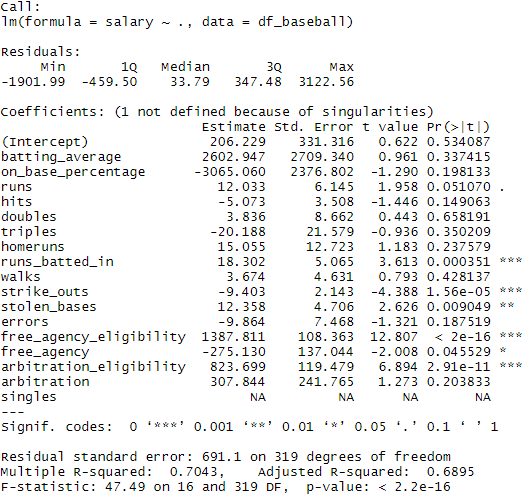
\includegraphics[scale=0.7]{images/multifit1.PNG}
\caption{Summary para el fit con todas las variables.}
\end{figure}

\begin{figure}[H]
\centering
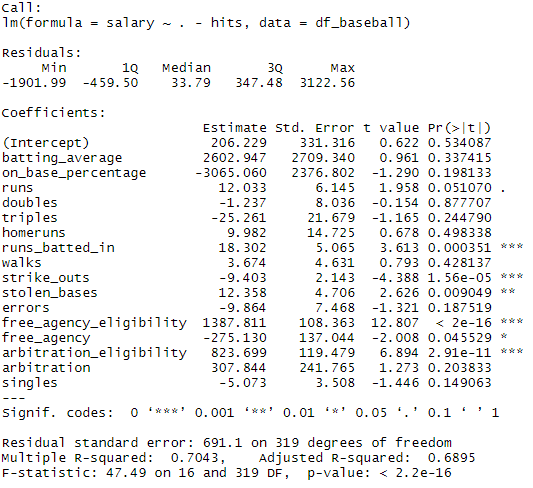
\includegraphics[scale=0.7]{images/multifit2.PNG}
\caption{Summary para la regresión lineal múltiple tras quitar \textit{``hits''}.}
\end{figure}

\begin{figure}[H]
\centering
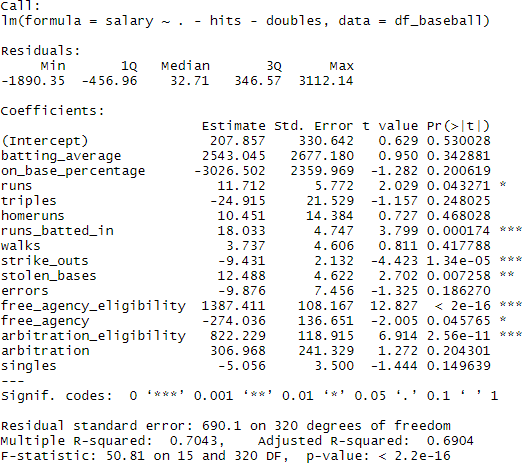
\includegraphics[scale=0.7]{images/multifit3.PNG}
\caption{Summary para la regresión lineal múltiple tras quitar \textit{``doubles''}.}
\end{figure}

\begin{figure}[H]
\centering
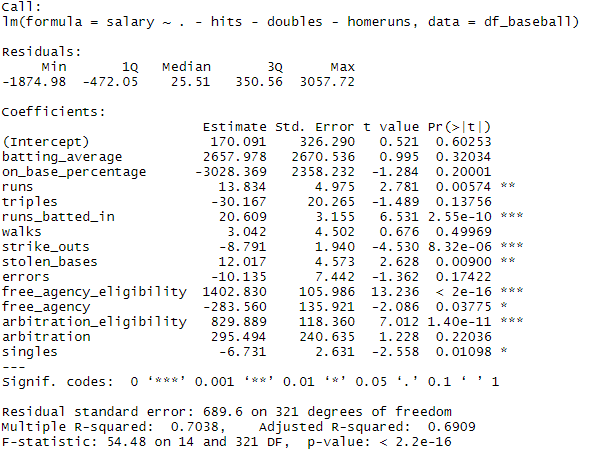
\includegraphics[scale=0.7]{images/multifit4.PNG}
\caption{Summary para la regresión lineal múltiple tras quitar \textit{``homeruns''}.}
\end{figure}

\begin{figure}[H]
\centering
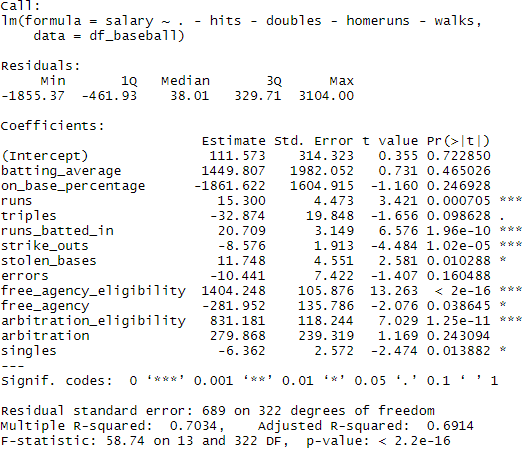
\includegraphics[scale=0.7]{images/multifit5.PNG}
\caption{Summary para la regresión lineal múltiple tras quitar \textit{``walks''}..}
\end{figure}

\begin{figure}[H]
\centering
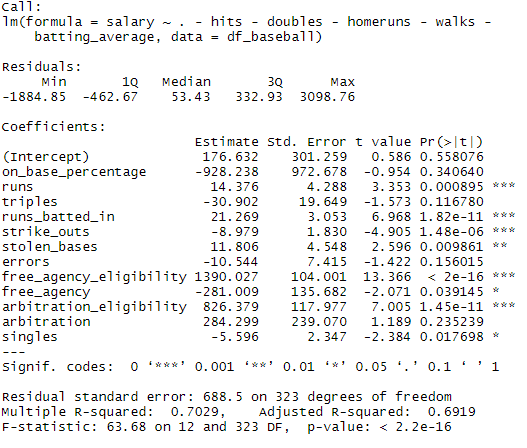
\includegraphics[scale=0.7]{images/multifit6.PNG}
\caption{Summary para la regresión lineal múltiple tras quitar \textit{``batting\_average''}..}
\end{figure}

\begin{figure}[H]
\centering
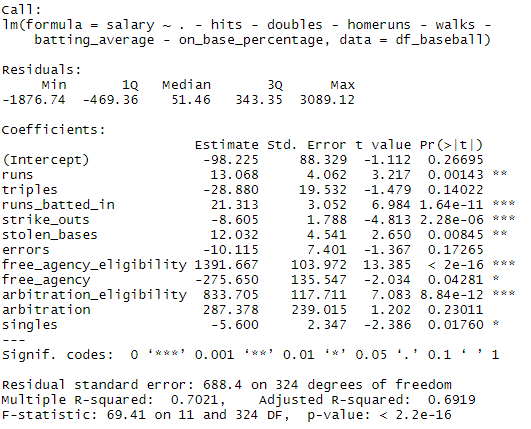
\includegraphics[scale=0.7]{images/multifit7.PNG}
\caption{Summary para la regresión lineal múltiple tras quitar \textit{``on\_base\_percentage''}.}
\end{figure}

\begin{figure}[H]
\centering
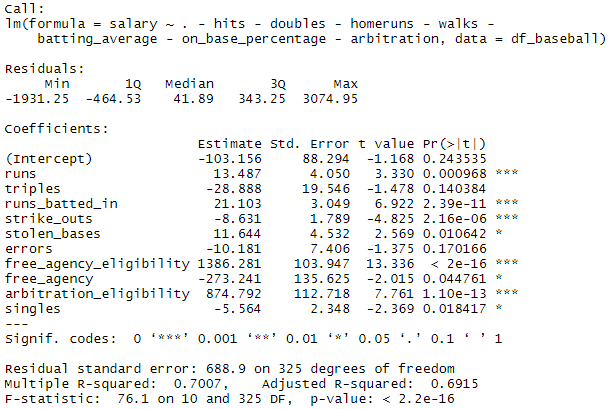
\includegraphics[scale=0.7]{images/multifit8.PNG}
\caption{Summary para la regresión lineal múltiple tras quitar \textit{``arbitration''}.}
\end{figure}

\begin{figure}[H]
\centering
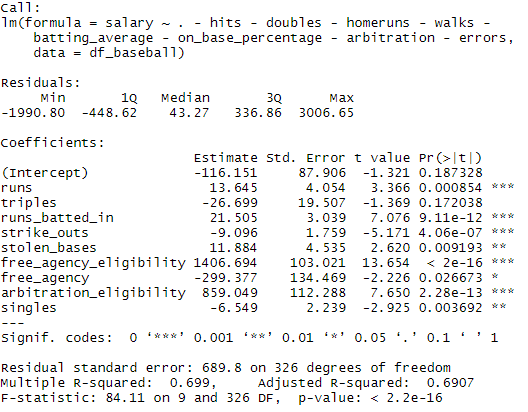
\includegraphics[scale=0.7]{images/multifit9.PNG}
\caption{Summary para la regresión lineal múltiple tras quitar \textit{``errors''}.}
\end{figure}

\begin{figure}[H]
\centering
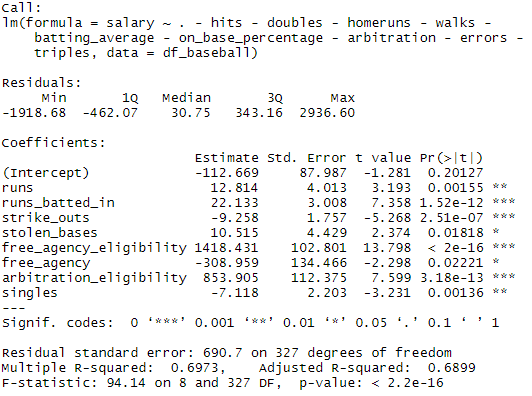
\includegraphics[scale=0.7]{images/multifit10.PNG}
\caption{Summary para la regresión lineal múltiple tras quitar \textit{``triples''}. Modelo más preciso.}
\end{figure}

\begin{figure}[H]
\centering
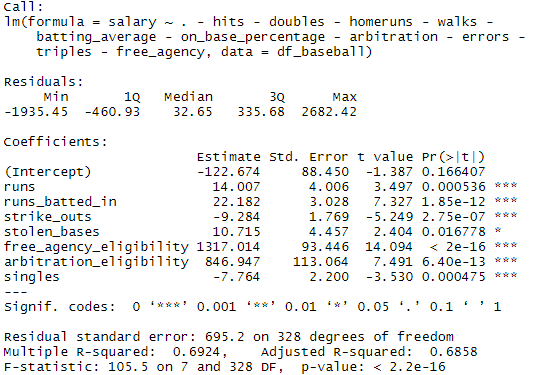
\includegraphics[scale=0.7]{images/multifit11.PNG}
\caption{Summary para la regresión lineal múltiple tras quitar \textit{``free\_agency''}.}
\end{figure}

\begin{figure}[H]
\centering
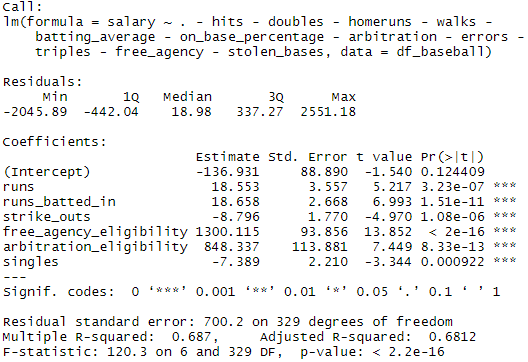
\includegraphics[scale=0.7]{images/multifit12.PNG}
\caption{Summary para la regresión lineal múltiple tras quitar \textit{``stolen\_bases''}.}
\end{figure}

\begin{figure}[H]
\centering
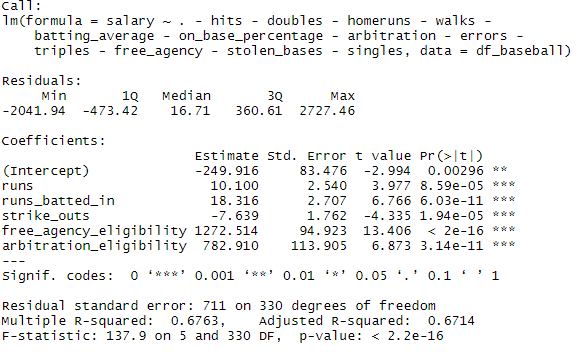
\includegraphics[scale=0.7]{images/multifit13.PNG}
\caption{Summary para la regresión lineal múltiple tras quitar \textit{``singles''}.}
\end{figure}

\begin{figure}[H]
\centering
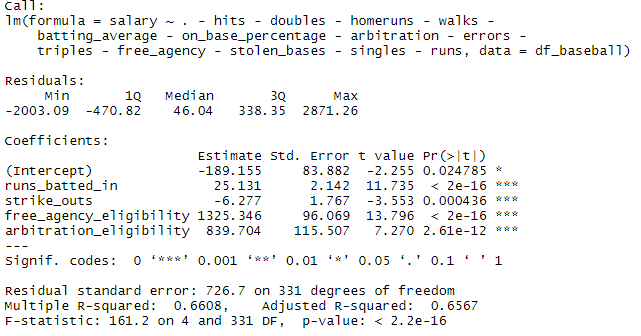
\includegraphics[scale=0.7]{images/multifit14.PNG}
\caption{Summary para la regresión lineal múltiple tras quitar \textit{``runs''}.}
\end{figure}

\begin{figure}[H]
\centering
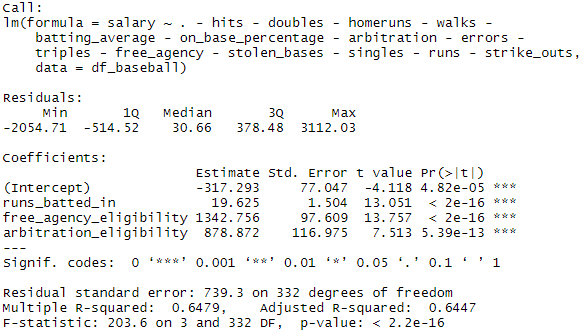
\includegraphics[scale=0.7]{images/multifit15.PNG}
\caption{Summary para la regresión lineal múltiple tras quitar \textit{``strike\_outs''}. Modelo más interpretable.}
\label{img:reginterpretable}
\end{figure}
El cambio del modelo presente en la figura anterior (\ref{img:reginterpretable}) a la próxima figura (\ref{img:reginterpretable2})
implica una disminución muy considerable de nuestro $R^2$ ajustado, pasando del 64.47 \% de explicación del error al 58.55 \% (una pérdida del casi 6 \%). Teniendo en cuenta que ya el número de variables era relativamente bajo pues sólo estamos pasando de 3 a 2, parece bastante razonable quedarnos con el modelo anterior e indagar si aplicar algún tipo de interacción o comportamiento no lineal nos permite mejorar los resultados obtenidos. \\

\begin{figure}[H]
\centering
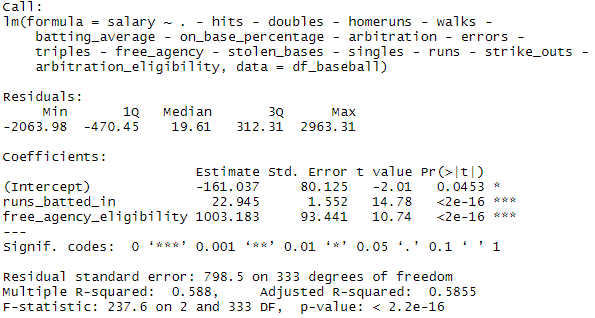
\includegraphics[scale=0.7]{images/multifit16.PNG}
\caption{Summary para la regresión lineal múltiple tras quitar \textit{``arbitration\_eligibility''}.}
\label{img:reginterpretable2}
\end{figure}

Nuestro objetivo ahora es, por tanto, probar algunas de estas transformaciones y ver si nuestros resultados mejoran o empeoran. Las tres variables que nos han quedado en el modelo más interpretable son un estadístico de rendimiento, \textit{runs\_batted\_in}, y dos mecanismos que nos indican en cierta manera la veteranía de los jugadores así como permiten que los jugadores puedan luchar por la competitividad de su salario: ser agente libre y la arbitración. Ser agente libre, permite que otros equipos intenten fichar al jugador y puede ocurrir si el contrato con su equipo ha finalizado o lleva más de 6 años jugando en la MLB. La arbitración es un proceso de mediación en el que el jugador argumenta por un salario, el equipo argumenta por otro pues ambas partes no se han puesto de acuerdo y una tercera parte determina quién lleva razón y, por tanto, el salario que van a recibir. Jugadores que llevan entre 3 y 6 años en la MLB pueden recurrir a ese mecanismo. El acceso a estos mecanismos viene representado por una categoría binaria en el dataset.\\


Durante el proceso del análisis exploratorio de datos, vimos mediante boxplots que la distribución del salario era superior en los casos que se tenían acceso a alguna de estas herramientas. Veamos gráficamente la influencia que tiene en el salario combinar estas categorías con el estadístico de rendimiento.

\begin{figure}[H]
\centering
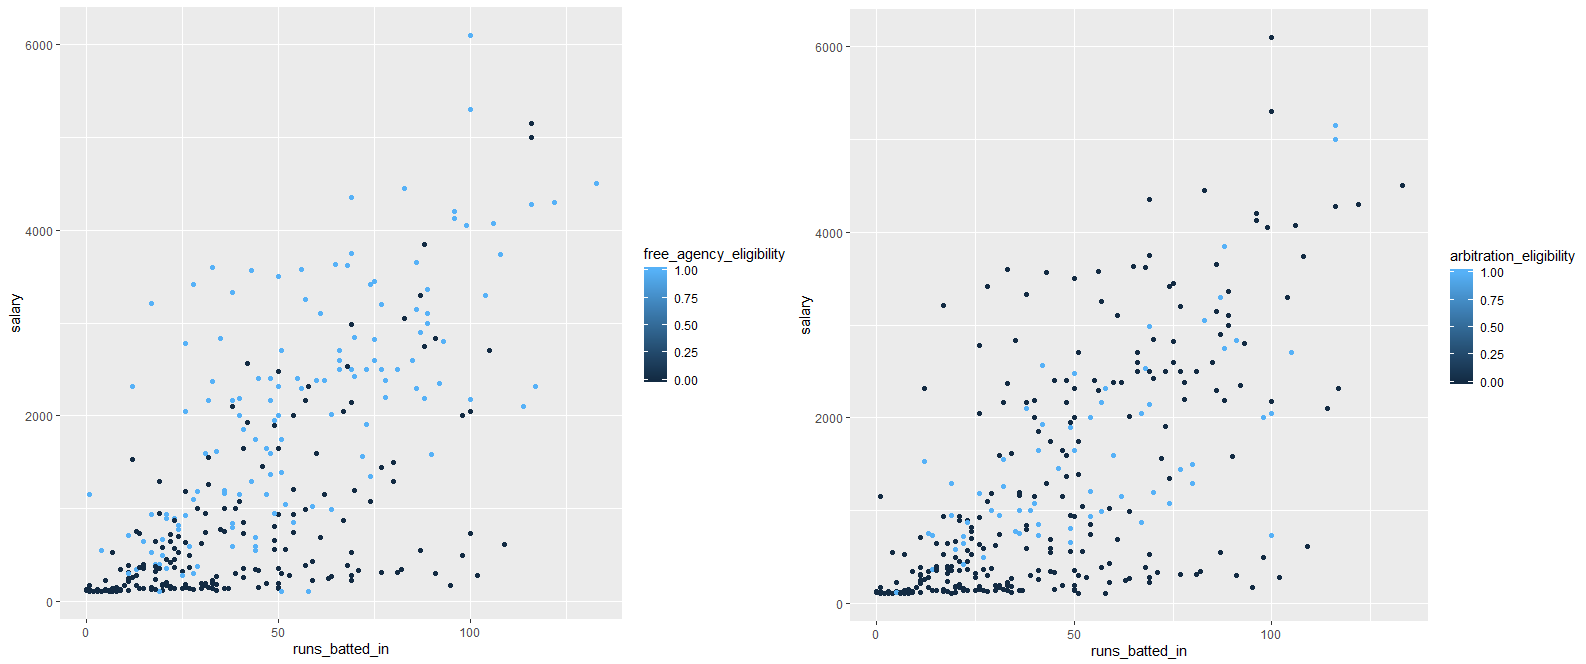
\includegraphics[scale=0.4]{images/rbi_agency.png}
\caption{Diagrama de dispersión del salario en función de RBI. El color indica el acceso a las herramientas.}
\end{figure}

Queda claro que acceder a alguno de esos mecanismos fomenta tener un mejor salario. De hecho, vamos a crear una nueva característica que va a consistir en la aplicación de la función lógica \textit{or} sobre ambas variables categóricas, mantendremos una de la dos variables originales y la otra la quitaremos pues estaría demasiado correlada similar a como nos ocurría con \textit{``hits''} y \textit{``singles''}. Veamos qué ocurre con el diagrama de dispersión coloreando los puntos con la nueva variable.

\begin{figure}[H]
\centering
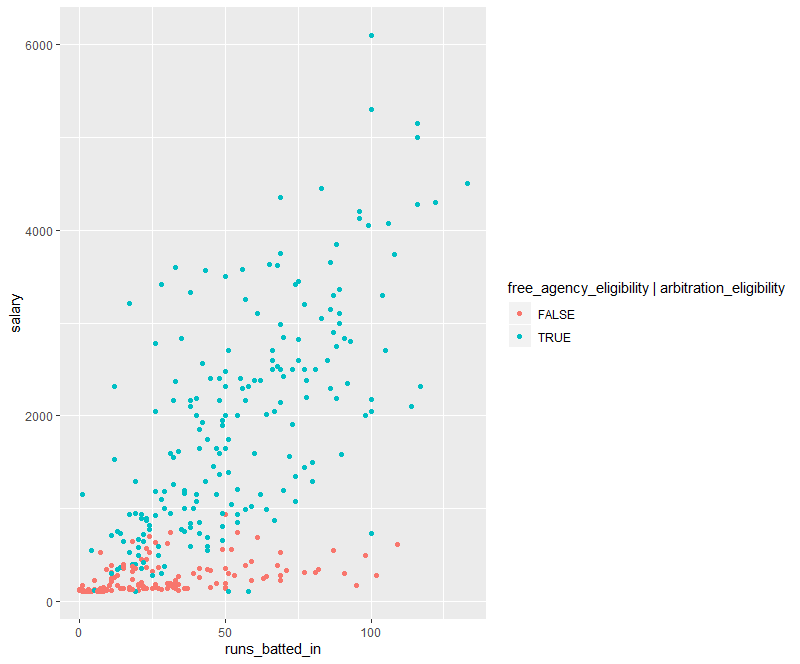
\includegraphics[scale=0.7]{images/competitivity_plot.png}
\caption{Diagrama de dispersión del salario en función de RBI. El color indica el acceso a alguna de las herramientas.}
\label{interpretregplot}
\end{figure}

El diagrama de dispersión de la figura anterior (\ref{interpretregplot}) y al que hemos llegado a través de la aplicación del método descendente y el uso de los conocimientos adquiridos en el análisis exploratorio de datos, nos permitir interpretar de una manera bastante clara qué está pasando con el conjunto de datos. En esa figura vemos cómo los jugadores que no tienen acceso a esos mecanismos para la competitividad de su salario rondan salarios cerca del mínimo independiente de su rendimiento. Por otro lado, para los jugadores que tienen acceso a esos mecanismos, los salarios aumentan conforme aumento su \textit{runs\_batted\_in}. Para estos últimos, podemos observar un comportamiento lineal aunque sujeto a varianzas altas. \\

De esta última gráfica, podemos sacar cuatro conclusiones:
\begin{itemize}
	\item La interacción entre \textit{runs\_batted\_in} y la función \textit{or} entre el acceso a ambos mecanismos (este \textit{or} va a quedar reflejado en la variable \textit{comp\_eligibility}) es posible que explique considerablemente mejor el salario.
	\item Un método lineal no va a poder explicar perfectamente la historia que estamos viendo en esta gráfica, necesitaríamos estudiar cada subproblema con un modelo lineal distinto o usar un método no lineal. (Uno de los subproblemas sería explicar el salario de los que tienen acceso a los mecanismos y el otro el salario de quien no puede utilizarlos)
	\item Aunque \textit{runs\_batted\_in} explique bastante bien a grandes rasgos qué esta pasando, puede que hayamos perdido alguna variable que quizás no tiene una relación lineal y requiere de alguna transformación que nos pueda permitir ayudar a mejorar la predicción de la varianza del salario.
	\item La relación entre \textit{runs\_batted\_in} y el salario parece ser exponencial. Aplicar una transformación logarítmica al salario podría mejorar los resultados aunque dificultaría la interpretabilidad del problema.
\end{itemize}

En primer lugar, vamos a probar a añadir la interacción propuesta entre \textit{runs\_batted\_in} y el salario.\\

\begin{figure}[H]
\centering
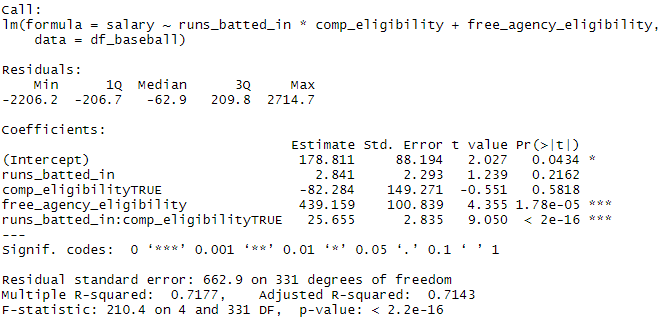
\includegraphics[scale=0.7]{images/multifitinter1.png}
\caption{Summary para modelo con la interacción propuesta entre RBI y mecanismos de competitividad.}
\end{figure}

Al añadir la interacción propuesta, obtenemos el mejor $R^2$ encontrado hasta el momento, del 71.43 \%. Probemos también a añadir la transformación logarítmica del salario.\\

\begin{figure}[H]
\centering
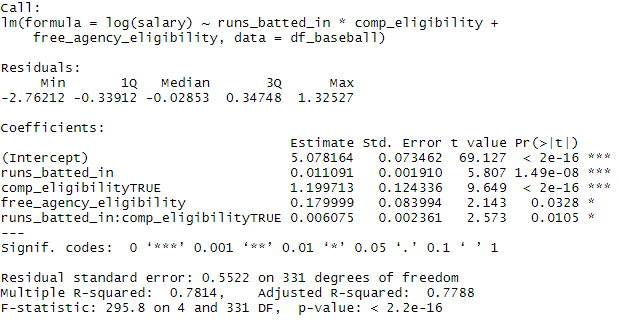
\includegraphics[scale=0.7]{images/summarylog.png}
\caption{Summary para modelo con transformación logarítmica del salario.}
\end{figure}

Otra vez conseguimos mejorar considerablemente el $R^2$ ajustado obtenido, hasta el 77,88 \%. Para finalizar, vamos a probar con la interacción entre \textit{``runs''} y \textit{``runs\_batted\_in''} pues por el propio nombre podemos intuir que ambas variables están relacionadas.

\begin{figure}[H]
\centering
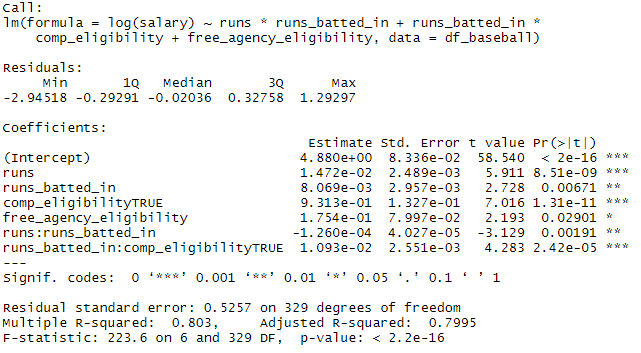
\includegraphics[scale=0.7]{images/runsinteract.png}
\caption{Summary para modelo con interacción entre \textit{``runs''} y \textit{``runs\_batted\_in''.}}
\end{figure}

Otra vez hemos conseguido un mejora del $R^2$ ajustado, hasta el 79,95 \%. Para comprobar cuál de los seleccionados es el mejor vamos a aplicar validación cruzada en los 5-\textit{folds} propuestos. Vamos a considerar el modelo más interpretable y el considerado más preciso sin las interacciones y la no linealidad así como todos los modelos con interacciones y no linealidad.

\begin{table}[H]
\centering
\footnotesize
\begin{tabular}{@{}lcccccc@{}}
\toprule
\multicolumn{1}{c}{\textbf{Modelo}} & \textbf{Fold 1} & \textbf{Fold 2} & \textbf{Fold 3} & \textbf{Fold 4} & \textbf{Fold 5} & \textbf{Media Fold} \\ \midrule
\textbf{Múltiple ``Preciso''} & 436755.8 & 564690.8 & 498310.6 & 484413.4 & 511764.7 & 499187.1 \\
\textbf{Múltiple ``Intepretable''} & 526498.3 & 566824.6 & 573202.3 & 608600.8 & 482814.1 & 551588 \\
\textbf{Anterior + rbi*comp\_eligibility} & 401753.3 & 595691 & \textbf{406162.7} & 463341.9 & 384432.3 & \textbf{450276.3} \\
\textbf{Anterior con log(salary)} & 344322.7 & 791816.2 & 520057.4 & 524848.7 & \textbf{458421} & 527893.2 \\
\textbf{Anterior + rbi*runs} & \textbf{343363.6} & \textbf{554903.2} & 436910.5 & 491825.4 & 435846.2 & 452569.8 \\ \bottomrule
\end{tabular}
\caption{Tabla resumen de MSE en validación cruzada aplicada a los modelos de regresión lineal múltiple.}
\label{tab:msemultireg}
\end{table}

El mejor modelo de regresión lineal múltiple que hemos obtenido es $salary \sim runs\_batted\_in*comp\_eligibility+free\_agency\_eligibility$. También es mejor que todos los modelos vistos de regresión lineal simple (teníamos los datos de la validación cruzada en las tablas).







\section[k-nn para regresión]{Aplicar el algoritmo k-nn para regresión.}
Para ver qué modelo funciona mejor con knn vamos a probar con los modelos propuestos en la regresión lineal múltiple y, además, vamos a probar con los valores de k 3, 5 y 7. El modelo que de mejor resultado en validación cruzada de 5-\textit{folds} (menor MSE) será con el que nos quedemos. La función utilizada se encarga de autoescalar las variables para que todas tengan la misma desviación estándar. Ademas los modelos previamente propuestos añadimos obtener el salario en función de todas las variables y obtener el logaritmo del salario en función de todas las variables. La siguiente tabla resumen recoge los resultado obtenidos para todos estos ajustes del modelo. El modelo múltiple que habíamos considerado como ``preciso'' al aplicar el método descendente en la regresión lineal múltiple es el que da mejores resultados con el knn (para un valor de k igual a 7). Este modelo sería $salary \sim runs + runs\_batted\_in + strike\_outs + stolen\_bases + free\_agency\_eligibility + free\_agency + arbitration\_eligibility + singles$ (MSE 487469.7). El mejor ajuste que hemos encontrado para knn en validación cruzada da peores resultados que el mejor que habíamos encontrado en regresión lineal múltiple (MSE 450276.3).

\begin{table}[H]
\centering
\footnotesize
\begin{tabular}{@{}lcccccc@{}}
\toprule
\multicolumn{1}{c}{\textbf{Modelo}} & \textbf{Fold 1} & \textbf{Fold 2} & \textbf{Fold 3} & \textbf{Fold 4} & \textbf{Fold 5} & \textbf{Media Fold} \\ \midrule
\multicolumn{7}{c}{\textbf{k=3}} \\
\textbf{Múltiple ``Preciso''} & 571659.9 & 712008.7 & 469093.3 & 481649.7 & 601349.6 & 567152.2 \\
\textbf{Múltiple ``Intepretable''} & 497421.4 & 763829.2 & 440190.8 & 597121 & 753399.7 & 610392.4 \\
\textbf{Anterior + rbi*comp\_eligibility} & 517219.9 & 768134.4 & 486296.8 & 558231.7 & 778398.1 & 621656.2 \\
\textbf{Anterior con log(salary)} & 518779.7 & 777555.8 & 497822.4 & 595916 & 754819.1 & 628978.6 \\
\textbf{Anterior + rbi*runs} & 618167 & 667278.1 & 590460 & 597495.4 & 612468.6 & 617173.8 \\
\textbf{salary $\sim$ .} & 657633.7 & 636843.5 & 548648.8 & 478283 & 712403.8 & 606762.6 \\
\textbf{log(salary) $\sim$ .} & 589888.5 & 629352.6 & 571951.8 & 489992.8 & 718445.5 & 599926.2 \\
\multicolumn{7}{c}{\textbf{k=5}} \\
\textbf{Múltiple ``Preciso''} & 512195.9 & 622044.2 & 403311.6 & 440596.4 & 577119.6 & 511053.5 \\
\textbf{Múltiple ``Intepretable''} & 421552.8 & 611207.9 & 435096.6 & 521347.6 & 753722.3 & 548585.4 \\
\textbf{Anterior + rbi*comp\_eligibility} & 411919.9 & 626228.2 & 430429.2 & 497560.9 & 709165.1 & 535060.7 \\
\textbf{Anterior con log(salary)} & \textbf{403288.8} & 628047.9 & 490734.6 & 551778.5 & 744298.8 & 563629.7 \\
\textbf{Anterior + rbi*runs} & 540197.8 & 625449.8 & 526478.9 & 588637.2 & 555195.2 & 567191.8 \\
\textbf{salary $\sim$ .} & 655673.8 & 562005 & 462676.1 & 478761.5 & 623208.5 & 556465 \\
\textbf{log(salary) $\sim$ .} & 567225.2 & 544586.2 & 526292.8 & 498194.7 & 625234.4 & 552306.6 \\
\multicolumn{7}{c}{\textbf{k=7}} \\
\textbf{Múltiple ``Preciso''} & 508500.4 & 568490 & \textbf{369075.6} & \textbf{422404.8} & 568877.9 & \textbf{487469.7} \\
\textbf{Múltiple ``Intepretable''} & 423734.8 & 570663.4 & 419660.2 & 503336.2 & 680693.6 & 519617.6\\
\textbf{Anterior + rbi*comp\_eligibility} & 429342.5 & 577570.1 & 422255.4 & 492496.5 & 689092.2 & 522151.3 \\
\textbf{Anterior con log(salary)} & 422781.3 & 589394.8 & 487816.3 & 558668.8 & 735324.2 & 558797.1 \\
\textbf{Anterior + rbi*runs} & 506634.6 & 616861.1 & 496602.9 & 564041.6 & \textbf{530299.3} & 542887.9 \\
\textbf{salary $\sim$ .} & 645339.2 & 524800.2 & 432253.9 & 472535.8 & 592036.7 & 533393.1 \\
\textbf{log(salary) $\sim$ .} & 546375.4 & \textbf{510960.5} & 530625.6 & 506173.8 & 596932.1 & 538213.5 \\ \bottomrule
\end{tabular}
\caption{Tabla resumen de MSE en validación cruzada aplicada a los modelos de regresión con knn.}
\label{tab:mseknnreg}
\end{table}

\newpage
\section[Comparativa de algoritmos]{Comparar los resultados de los dos algoritmos regresión múltiple entre sí, y adicionalmente mediante comparativas múltiples con un tercero (el modelo de regresión M5', cuyos resultados ya están incluidos en las tablas de resultados disponibles).}
Ahora vamos a comparar los algoritmos de regresión lineal múltiple, knn y M5'. Para ello, vamos a utilizar las tablas con los resultados obtenidos en train y test de estos algoritmos sobre un conjunto de datasets que nos han proporcionado. Los resultados concretos para el dataset con el que estamos trabajando ``baseball'' serán sustituidos por los del modelo general (incluir todas las variables, sin las añadidas por mí que podría generar colinealidades) en la validación cruzada de 5 folds en test. El de M5' quedará sin modificarse pues no hemos aplicado ese algoritmo. \\

En primer lugar, vamos a ver si existen diferencias significativas entre regresión lineal múltiple y knn. Para ello, utilizamos el test de Wilcoxon. El test de Wilcoxon es un test no paramétrico que nos permite determinar si dos muestras dependientes están relacionadas. A la hora de comparar dos clasificadores, estamos comparando las medidas de precisión del algoritmo (en nuestro caso MSE) para los distintos modelos en cada dataset, por lo que si una muestra esta conformada por un dataset, las medidas de precisión de cada algoritmo son variables relacionadas. Si el p-value está por debajo del nivel de significancia (para este experimento lo vamos a fijar a 0.05), rechazamos la hipótesis nula del test, lo que indicaría que uno de los modelos daría resultados significativamente distintos al del otro.

\begin{table}[H]
\centering
\begin{tabular}{@{}ccc@{}}
\toprule
R+ & R- & p-value \\ \midrule
77 & 94 & 0.7637265 \\ \bottomrule
\end{tabular}
\caption{Resultados de aplicar el test de Wilcoxon para comparar los algoritmos de regresión lineal y el knn para regresión.}
\label{tab:wilcoxreg}
\end{table}

Puesto que el \textit{p-value} es superior al nivel de significancia no podemos rechazar que ambos algoritmos ofrecen resultados similares. Ahora vamos a ver si existen diferencias significativas entre los 3 algoritmos, para ello aplicamos el test de Friedman.

\begin{table}[H]
\centering
\begin{tabular}{@{}ccc@{}}
\toprule
$\chi^2$ & df & p-value \\ \midrule
7.4444 & 2 & 0.02418 \\ \bottomrule
\end{tabular}
\caption{Resultados de aplicar el test de Friedman para comparar los 3 algoritmos.}
\label{tab:friedmanreg}
\end{table}
Puesto que el \textit{p-value} es inferior al nivel de significancia rechazamos la hipótesis nula, es decir, rechazamos que todos los algoritmos tienen una mediana de MSE similares. Ahora vamos a aplica un post-hoc Holm para ver qué pares de algoritmos pueden considerar similares.

\begin{table}[H]
\centering
\begin{tabular}{@{}ccc@{}}
\toprule
\multicolumn{1}{l}{Algoritmo} & \multicolumn{1}{l}{Regresión lineal} & \multicolumn{1}{l}{knn(Reg)} \\ \midrule
knn (Reg) & 0.424 & - \\
M5' & 0.081 & 0.424 \\ \bottomrule
\end{tabular}
\caption{Test de wilcoxon por pares. Post-hoc Holm.}
\label{tab:friedmanreg}
\end{table}

Existen diferencias significativas a favor de M5' con respecto a la regresión lineal. Los otros pares pueden ser considerados equivalentes.

\chapter{Clasificación.}
\textit{Nota: Del EDA hemos optado por discretizar la variable número de hijos en cero, uno, dos y tres, cuatro o más. Además, todas las variables categóricas son ordenadas y han sido convertidas en factores ordenados.}

\section[k-NN para clasificación.]{Utilizar el algoritmo k-NN probando con diferentes valores de k. Elegir el que considere más adecuado para su conjunto de datos. Analice qué ocurre en los valores de precisión en training y test con los diferentes valores de k.}

Para utilizar knn, vamos a usar la librería \textit{kknn}. Esta librería nos ofrece la función kknn, que nos permite entrenar el modelo indicándole mediante una fórmula qué variable predecir y qué variables usar como predictores, el número de vecinos más cercanos, la partición de training y test y el valor de la distancia de Minkowski. Vamos a considerar utilizar la distancia de Manhattan y la distancia euclídea y vamos a probar todos los valores posibles de k desde 1 hasta 20, ignorando aquellos que sean múltiplos de 3. La función usada se encarga automáticamente de escalar las variables para que todas tengan la misma desviación típica. La siguiente tabla resumen representa los resultados obtenidos al ejecutar knn sobre nuestro conjunto en las particiones propuestas.\\

\scriptsize	
\begin{longtable}{@{}cccccccccccc@{}}
\toprule
 & \textbf{Fold 1} & \textbf{Fold 2} & \textbf{Fold 3} & \textbf{Fold 4} & \textbf{Fold 5} & \textbf{Fold 6} & \textbf{Fold 7} & \textbf{Fold 8} & \textbf{Fold 9} & \textbf{Fold 10} & \textbf{Media} \\* \midrule
\endhead
%
\bottomrule
\endfoot
%
\endlastfoot
%
\textbf{k=1 (E)} & 0.419 & 0.446 & 0.392 & 0.388 & 0.463 & 0.469 & 0.435 & 0.435 & 0.476 & 0.422 & 0.435 \\
\textbf{k=2 (E)} & 0.432 & 0.459 & 0.392 & 0.388 & 0.469 & 0.503 & 0.422 & 0.442 & 0.483 & 0.422 & 0.441 \\
\textbf{k=4 (E)} & 0.426 & 0.459 & 0.392 & 0.395 & 0.463 & 0.483 & 0.422 & 0.456 & 0.483 & 0.422 & 0.440 \\
\textbf{k=5 (E)} & 0.453 & 0.486 & 0.412 & 0.401 & 0.483 & 0.531 & 0.435 & 0.463 & 0.469 & 0.415 & 0.455
 \\
\textbf{k=7 (E)}   & 0.473 & 0.493 & 0.412 & 0.442 & 0.503 & 0.531 & 0.463 & 0.483 & 0.483 & 0.435 & 0.472
\\
\textbf{k=8 (E)}   & 0.500 & 0.500 & 0.412 & 0.463 & 0.476 & 0.517 & 0.442 & 0.517 & 0.497 & 0.442 & 0.477
\\
\textbf{k=10 (E)}   & 0.507 & 0.486 & 0.439 & 0.469 & 0.490 & 0.531 & 0.456 & 0.469 & 0.524 & 0.449 & 0.482
\\
\textbf{k=11 (E)}  & 0.507 & 0.493 & 0.439 & 0.476 & 0.497 & 0.537 & 0.442 & 0.497 & 0.531 & 0.469 & 0.489
 \\
\textbf{k=13 (E)}   & 0.514 & 0.500 & 0.453 & 0.483 & 0.510 & 0.544 & 0.449 & 0.524 & 0.524 & 0.463 & 0.496
\\
\textbf{k=14 (E)}  & 0.507 & 0.493 & 0.439 & 0.476 & 0.497 & 0.551 & 0.469 & 0.517 & 0.524 & 0.463 & 0.494
 \\
\textbf{k=16 (E)}   & 0.493 & 0.507 & 0.439 & 0.476 & 0.510 & 0.544 & 0.497 & 0.517 & 0.524 & 0.469 & 0.498
\\
\textbf{k=17 (E)}   & 0.500 & 0.507 & 0.459 & 0.483 & 0.517 & 0.565 & 0.476 & 0.537 & 0.537 & 0.463 & 0.504
\\
\textbf{k=19 (E)}  & 0.507 & \textbf{0.514} & 0.459 & 0.476 & \textbf{0.524} & 0.558 & 0.456 & 0.531 & 0.537 & 0.449 & 0.501
 \\
\textbf{k=20 (E)}  & 0.493 & 0.507 & 0.453 & 0.476 & 0.517 & 0.565 & 0.463 & \textbf{0.537} & 0.524 & 0.463 & 0.500
 \\
\textbf{k=1 (M)}   & 0.432 & 0.446 & 0.399 & 0.388 & 0.435 & 0.463 & 0.415 & 0.456 & 0.469 & 0.442 & 0.435
\\
\textbf{k=2 (M)}   & 0.453 & 0.473 & 0.392 & 0.374 & 0.449 & 0.503 & 0.408 & 0.463 & 0.463 & 0.435 & 0.441
\\
\textbf{k=4 (M)}  & 0.432 & 0.453 & 0.392 & 0.374 & 0.449 & 0.469 & 0.408 & 0.469 & 0.469 & 0.435 & 0.435
 \\
\textbf{k=5 (M)}   & 0.439 & 0.459 & 0.399 & 0.422 & 0.483 & 0.517 & 0.408 & 0.497 & 0.463 & 0.442 & 0.453
\\
\textbf{k=7 (M)}   & 0.466 & 0.480 & 0.426 & 0.469 & 0.497 & 0.510 & 0.415 & 0.517 & 0.483 & 0.449 & 0.471
\\
\textbf{k=8 (M)}   & 0.480 & 0.473 & 0.405 & 0.483 & 0.490 & 0.510 & 0.429 & 0.524 & 0.476 & \textbf{0.483} & 0.475
\\
\textbf{k=10 (M)}  & 0.486 & 0.473 & 0.432 & 0.476 & 0.497 & 0.537 & 0.449 & 0.503 & 0.497 & 0.469 & 0.482
 \\
\textbf{k=11 (M)}   & 0.486 & 0.473 & 0.439 & \textbf{0.503} & 0.497 & 0.544 & 0.449 & 0.510 & 0.510 & 0.476 & 0.489
\\
\textbf{k=13 (M)}   & 0.507 & 0.480 & 0.446 & 0.490 & 0.497 & 0.571 & 0.483 & 0.544 & 0.531 & 0.476 & 0.502
\\
\textbf{k=14 (M)}  & 0.500 & 0.500 & 0.446 & 0.497 & 0.497 & 0.571 & 0.483 & 0.544 & 0.544 & 0.463 & 0.504
 \\
\textbf{k=16 (M)}  & 0.520 & 0.500 & 0.459 & 0.483 & 0.490 & 0.565 & \textbf{0.503} & 0.531 & 0.565 & 0.463 & \textbf{0.508}
 \\
\textbf{k=17 (M)}   & 0.514 & 0.493 & \textbf{0.466} & 0.469 & 0.490 & 0.571 & 0.497 & 0.531 & \textbf{0.571} & 0.449 & 0.505
\\
\textbf{k=19 (M)}   & 0.527 & 0.500 & \textbf{0.466} & 0.463 & 0.497 & 0.571 & 0.490 & 0.517 & 0.558 & 0.463 & 0.505
\\
\textbf{k=20 (M)}  & \textbf{0.534} & 0.500 & 0.459 & 0.456 & 0.497 & \textbf{0.578} & 0.476 & 0.531 & 0.558 & 0.463 & 0.505 \\* \bottomrule
\caption{Resumen de los resultados de validación cruzada con knn.}
\label{tab:knnclass}\\


\end{longtable}
\normalsize
El mejor resultado lo hemos obtenido utilizando knn con un 50,8 \% de precisión usando la distancia Manhattan con k=16 vecinos más cercanos.

\section[LDA para clasificación.]{Utilizar el algoritmo LDA para clasificar. No olvide comprobar las asunciones.}
El algoritmo LDA asume normalidad de las variables con las que trabajamos. Para comprobar la normalidad, vamos a aplicar el test de Shapiro-Wilk para normalidad de nuestras variables. Gran parte de las variables con las que trabajamos son de estilo categórico, así que vamos a pasarla a numérica y aplicar el test, aunque lo habitual sería que no siga una distribución normal.\\

Como podemos observar todos los p-values son inferiores a 2.2e-16, por lo que se rechaza la hipótesis nula de que la variable siga una distribución normal. Aunque esta premisa no se cumpla, vamos a aplicar el método LDA con todas las variables y ver qué resultados obtenemos.\\

Además, el método también asume que todas las variables siguen una varianza similar y que las variables sean independientes. Como podemos observar en la tabla mostrada a continuación, esta premisa tampoco se cumple.\\

\begin{table}[H]
\centering
\begin{tabular}{@{}lccc@{}}
\toprule
\multicolumn{1}{c}{\textbf{Variable}} & \textbf{W} & \textbf{p-value} & \multicolumn{1}{l}{\textbf{Varianza}} \\ \midrule
\textbf{wife\_age} & 0.96571 & \textless{}2.2e-16 & 67.688 \\
\textbf{wife\_education} & 0.80447 & \textless{}2.2e-16 & 1.462 \\
\textbf{husband\_education} & 0.69839 & \textless{}2.2e-16 & 1.317 \\
\textbf{wife\_religion} & 0.42536 & \textless{}2.2e-16 & 0.127 \\
\textbf{wife\_working} & 0.53895 & \textless{}2.2e-16 & 0.188 \\
\textbf{husband\_occupation} & 0.81491 & \textless{}2.2e-16 & 0.748\\
\textbf{standard\_of\_living} & 0.78287 & \textless{}2.2e-16 & 1.36 \\
\textbf{media\_exposure} & 0.28639 & \textless{}2.2e-16 & 0.069 \\
\textbf{children.cat} & 0.78133 & \textless{}2.2e-16 & 0.998\\
\textbf{contraceptive\_method} & 0.78369 & \textless{}2.2e-16 & 0.613 \\ \bottomrule
\end{tabular}
\caption{Test de normalidad de Shapiro-Wilk y varianzas de las variables.}
\label{tab:shapironormality}
\end{table}

Para ejecutar LDA, utilizamos la función lda del paquete MASS. Esta función, como ocurría en kknn, nos permite usar una fórmula para determinar qué variable queremos predecir y cuáles usar como predictores. Tanto en el caso de LDA como QDA nos hemos limitado a usar todas las variables, aunque quizás sería de interés probar múltiples configuraciones con diferentes conjuntos de variables. A la hora de ejecutarlo realizamos validación cruzada usando lda sobre todas las variables. Los resultados obtenidos, en términos de precisión, son los siguientes: \\

\begin{table}[H]
\centering
\begin{tabular}{@{}lc@{}}
\toprule
\multicolumn{1}{c}{\textbf{LDA}} & \textbf{Precisión} \\ \midrule
\textbf{Fold 1} & 0.514 \\
\textbf{Fold 2} & 0.466 \\
\textbf{Fold 3} & 0.439 \\
\textbf{Fold 4} & 0.537 \\
\textbf{Fold 5} & 0.503 \\
\textbf{Fold 6} & 0.558 \\
\textbf{Fold 7} & 0.517 \\
\textbf{Fold 8} & 0.524 \\
\textbf{Fold 9} & 0.435 \\
\textbf{Fold 10} & 0.510 \\
\textbf{Media} & 0.500 \\ \bottomrule
\end{tabular}
\caption{Resultados de validación cruzada con todas las variables en LDA.}
\label{tab:lda}
\end{table}



\section[QDA para clasificación.]{Utilizar el algoritmo QDA para clasificar. No olvide comprobar las asunciones.}
QDA tiene unas asunciones similares a las de LDA, excepto que ahora la varianza y covarianza se tienen en cuenta respecto a cada clase a predecir. Veamos si así se cumple:

\begin{table}[H]
\begin{tabular}{@{}lccc@{}}
\toprule
\multicolumn{1}{c}{\textbf{Variable}} & \textbf{Varianza (Clase 1)} & \textbf{Varianza (Clase 2)} & \textbf{Varianza (Clase 3)} \\ \midrule
\textbf{wife\_age} & 55.575 & 48.217 & 83.24 \\
\textbf{wife\_education} & 1.285 & 1.479 & 1.365 \\
\textbf{husband\_education} & 0.840 & 1.316 & 1.424 \\
\textbf{wife\_religion} & 0.177 & 0.117 & 0.105 \\
\textbf{wife\_working} & 0.196 & 0.169 & 0.198 \\
\textbf{husband\_occupation} & 0.785 & 0.704 & 0.705 \\
\textbf{standard\_of\_living} & 1.220 & 1.375 & 1.360 \\
\textbf{media\_exposure} & 0.029 & 0.047 & 0.104 \\
\textbf{children.cat} & 0.793 & 0.719 & 1.203 \\ \bottomrule
\end{tabular}
\caption{Varianzas de las variables según clase}
\label{tab:checkqda}
\end{table}

Para ejecutar QDA, utilizamos la función qda del paquete MASS. Igual que en el caso del lda, podemos determinar con una fórmula que variable predecir y que variables usar para la predicción mediante una fórmula. Los resultados obtenidos en validación cruzada, usando todas las variables para entrenar QDA son los siguientes:
\begin{table}[H]
\centering
\begin{tabular}{@{}lc@{}}
\toprule
\multicolumn{1}{c}{\textbf{QDA}} & \textbf{Precisión} \\ \midrule
\textbf{Fold 1} & 0.547 \\
\textbf{Fold 2} & 0.486 \\
\textbf{Fold 3} & 0.480 \\
\textbf{Fold 4} & 0.510 \\
\textbf{Fold 5} & 0.531 \\
\textbf{Fold 6} & 0.578 \\
\textbf{Fold 7} & 0.503 \\
\textbf{Fold 8} & 0.537 \\
\textbf{Fold 9} & 0.449 \\
\textbf{Fold 10} & 0.469 \\
\textbf{Media} & 0.509 \\ \bottomrule
\end{tabular}
\caption{Resultados de validación cruzada con todas las variables en QDA}
\label{tab:qda}
\end{table}
\section[Comparación de algoritmos.]{Comparar los resultados de los tres algoritmos.}

Por regla general, los algoritmos nos dan valores bastante similares en términos de precisión, aunque el mejor lo hemos encontrado en el uso de knn (aunque hemos de tener en cuenta que en este es el único en el que hemos probado varias configuraciones). Si nos basamos sólo en términos de precisión, el mejor modelo obtenido lo hemos encontrado usando la distancia Manhattan con k=16 (50,8 \%) de precisión. Por regla general, el nivel de acierto es bastante bajo si bien es cierto que no hemos aplicado ninguna técnica para resolver el problema de clasificación desbalanceada presente en el dataset y podría ser posible que nuestras variables no contengan suficiente información para generar una buena clasificación.\\

Para determinar si realmente existen diferencias significativas entre los tres modelos creados vamos a aplicar test estadísticos. Vamos a trabajar con los 10 valores de precisión obtenidos en cada uno de los casos. No vamos a realizar un test de normalidad pues el número de muestras con el que vamos a trabajar es muy pequeño así que directamente vamos a usar test no paramétricos. Por otro lado, nos encontramos ante un caso de medidas repetidas (1 medida de cada modelo para cada fold), así que aplicamos el test de Friedman para determinar si existen diferencias significativas entre, al menos, un par de algoritmos. \\

\begin{table}[H]
\centering
\begin{tabular}{@{}ccc@{}}
\toprule
$\chi^2$ & df & p-value \\ \midrule
3.2308 & 2 & 0.1988 \\ \bottomrule
\end{tabular}
\caption{Resultados de aplicar el test de Friedman para comparar los 3 modelos.}
\label{tab:friedmanclass}
\end{table}

Al salirnos un p-value superior a 0.05 no podemos rechazar la hipótesis nula de que las medianas de los algoritmos sean similares. En definitiva, los 3 modelos obtenidos nos ofrecen resultados similares para el problema con el que hemos trabajado.\\

Para finalizar, con el fin de entender si tenemos algún tipo de problema de sobreajuste que explique los malos resultados obtenidos miramos sus valores de precisión en training en los 3 modelos seleccionados.\\

\begin{table}[H]
\centering
\begin{tabular}{@{}lccc@{}}
\toprule
{}&{\textbf{KNN}} & \textbf{LDA} & \textbf{QDA}\\ \midrule
\textbf{Fold 1} & 0.7184906 & 0.5101887   & 0.5222642\\
\textbf{Fold 2} & 0.7252830 & 0.5222642   & 0.5283019\\
\textbf{Fold 3} & 0.7245283 & 0.5139623   & 0.5305660\\
\textbf{Fold 4} & 0.7254902 & 0.5128205   & 0.5203620\\
\textbf{Fold 5} & 0.7307692 & 0.5082956   & 0.5150830\\
\textbf{Fold 6} & 0.7164404 & 0.4984917   & 0.5196078\\
\textbf{Fold 7} & 0.7285068 & 0.5082956   & 0.5233786\\
\textbf{Fold 8} & 0.7232278 & 0.5082956   & 0.5256410\\
\textbf{Fold 9} & 0.7217195 & 0.5188537   & 0.5286576\\
\textbf{Fold 10} & 0.7262443 & 0.5045249  &  0.5279035\\\bottomrule
\end{tabular}
\caption{Comparación de valores de precisión en training.}
\label{tab:acctraining}
\end{table}

De esta última tabla podemos observar que no estamos incurriendo en un problema de sobreajuste pues la precisión en training es bastante similar a los resultados obtenidos en test (excepto en knn por el propio funcionamiento del mismo, estamos guardando las muestras de training para determinar los vecinos más cercanos y eso explica un mayor valor de precisión para el conjunto de training). Probablemente pasos apropiados para afrontar este problema deberían ser intentar solventar en la medida de lo posible el problema de clasificación desbalanceada, haría falta probar con una mayor diversidad de clasificadores y existe la posibilidad de que nuestros datos no sean lo suficientemente buenos para resolver el problema de clasificación.\\
\appendix
\chapter{Código Fuente de Análisis Exploratorio de Datos.}
\section{EDA dataset de regresión ``baseball''.}
\begin{minted}{r}
# Paquetes
library(VIM)
library(dplyr)
library(ggplot2)
library(corrplot)
# Leer dataset
df_baseball <- read.csv("baseball.dat", comment.char="@", header=F)
colnames(df_baseball) <- c("batting_average", "on_base_percentage", "runs",
	"hits", "doubles", "triples", "homeruns", "runs_batted_in", "walks", 
	"strike_outs", "stolen_bases", "errors",  "free_agency_eligibility", 
	"free_agency", "arbitration_eligibility", "arbitration", "salary")

# Comprobar tipos de datos
class(df_baseball)
apply(df_baseball, 2, class)
dim(df_baseball)

# Pasamos a factor
df_baseball$free_agency_eligibility <- as.factor(df_baseball$free_agency_eligibility)
df_baseball$free_agency <- as.factor(df_baseball$free_agency)
df_baseball$arbitration_eligibility <- as.factor(df_baseball$arbitration)
df_baseball$arbitration <- as.factor(df_baseball$arbitration)

# Medidas de tendencia central y dispersión
apply(df_baseball[-(13:16)], 2, min, na.rm=T)
apply(df_baseball[-(13:16)], 2, max, na.rm=T)
apply(df_baseball[-(13:16)], 2, mean, na.rm=T)
apply(df_baseball[-(13:16)], 2, median, na.rm=T)
apply(df_baseball[-(13:16)], 2, sd, na.rm=T)
apply(df_baseball[-(13:16)], 2, mad, na.rm=T)

# DETECCIÓN DE MUESTRAS DUPLICADAS
df_baseball[duplicated(df_baseball),]
# DETECCIÓN DE MISSING VALUES
aggr(df_baseball, col=c('blue','red'), numbers=TRUE,
 sortVars=TRUE, labels=names(df_baseball), cex.axis=.7, gap=3,
 ylab=c("Histogram of missing data","Pattern"))

# Qué pasa con los valores 0
df_baseball %>% filter(hits==1)
df_baseball %>% filter(strike_outs==1)
df_baseball %>% filter(runs==0)

# TABLAS DE CONTIGENCIA
table(df_baseball$free_agency_eligibility)
table(df_baseball$free_agency)
table(df_baseball$arbitration_eligibility)
table(df_baseball$arbitration)


# GENERACIÓN DE HISTOGRAMAS PARA VARIABLES CONTINUAS
ggplot(df_baseball, aes(x=batting_average)) + 
  geom_histogram(aes(y=..density..), binwidth = 0.005, color="blue", fill="green") +
  ggtitle("Histograma de batting_average (binwidth 0.005)") + ylab("densidad") + 
  geom_density(color="darkred")
## ------------------------------------------------------------------------
ggplot(df_baseball, aes(x=on_base_percentage)) + 
  geom_histogram(aes(y=..density..), binwidth = 0.005, color="blue", fill="green") +
  ggtitle("Histograma de on_base_percentage (binwidth 0.005)") + ylab("densidad") + 
  geom_density(color="darkred")
## ------------------------------------------------------------------------
ggplot(df_baseball, aes(x=runs)) + 
  geom_histogram(aes(y=..density..), bins=40, color="blue", fill="green") +
  ggtitle("Histograma de runs (40 bins)") + ylab("densidad") + 
  geom_density(color="darkred")
## ------------------------------------------------------------------------
ggplot(df_baseball, aes(x=hits)) + 
  geom_histogram(aes(y=..density..), bins=60, color="blue", fill="green") +
  ggtitle("Histograma de hits (60 bins)") + ylab("densidad") +
  geom_density(color="darkred")
## ------------------------------------------------------------------------
ggplot(df_baseball, aes(x=doubles)) + 
  geom_histogram(aes(y=..density..), bins=40, color="blue", fill="green") +
  ggtitle("Histograma de doubles (40 bins)") + ylab("densidad") + 
  geom_density(color="darkred")
## ------------------------------------------------------------------------
ggplot(df_baseball, aes(x=triples)) + 
  geom_histogram(aes(y=..density..), bins=15, color="blue", fill="green") +
  ggtitle("Histograma de triples (15 bins)") + ylab("densidad") + 
  geom_density(color="darkred")
## ------------------------------------------------------------------------
ggplot(df_baseball, aes(x=homeruns)) + 
  geom_histogram(aes(y=..density..), bins=40, color="blue", fill="green") +
  ggtitle("Histograma de homeruns (40 bins)") + ylab("densidad") + 
  geom_density(color="darkred")
## ------------------------------------------------------------------------
ggplot(df_baseball, aes(x=runs_batted_in)) + 
  geom_histogram(aes(y=..density..), bins=40, color="blue", fill="green") +
  ggtitle("Histograma de runs_batted_in (40 bins)") + ylab("densidad") + 
  geom_density(color="darkred")
## ------------------------------------------------------------------------
ggplot(df_baseball, aes(x=walks)) + 
  geom_histogram(aes(y=..density..), bins=50, color="blue", fill="green") +
  ggtitle("Histograma de walks (50 bins)") + ylab("densidad") + 
  geom_density(color="darkred")
## ------------------------------------------------------------------------
ggplot(df_baseball, aes(x=strike_outs)) + 
  geom_histogram(aes(y=..density..), bins=50, color="blue", fill="green") +
  ggtitle("Histograma de strike_outs (50 bins)") + ylab("densidad") + 
  geom_density(color="darkred")
## ------------------------------------------------------------------------
ggplot(df_baseball, aes(x=stolen_bases)) + 
  geom_histogram(aes(y=..density..), bins=30, color="blue", fill="green") +
  ggtitle("Histograma de stolen_bases (30 bins)") + ylab("densidad") + 
  geom_density(color="darkred")
## ------------------------------------------------------------------------
ggplot(df_baseball, aes(x=errors)) +
  geom_histogram(aes(y=..density..), bins=30, color="blue", fill="green") +
  ggtitle("Histograma de errors (30 bins)") + ylab("densidad") + 
  geom_density(color="darkred")
## ------------------------------------------------------------------------
ggplot(df_baseball, aes(x=salary)) + 
  geom_histogram(aes(y=..density..), bins=40, color="blue", fill="green") +
  ggtitle("Histograma de salary (40 bins)") + ylab("densidad") + 
  geom_density(color="darkred")

## Añadimos la varable singles
df_baseball <- df_baseball %>% mutate(singles=hits - doubles - triples - homeruns)

## Vemos si hay muestras erróneas
df_baseball %>% filter(singles < 0)

## Quitamos muestras erróneas-
df_baseball <- df_baseball %>% filter(!(singles < 0))

# 10 números más alto de singles para
# croroborar con fuente externa
df_baseball %>% arrange(desc(singles)) %>% select(singles) %>% head(10)
## HISTOGRAMA de singles
ggplot(df_baseball, aes(x=singles)) + 
  geom_histogram(aes(y=..density..), bins=50, color="blue", fill="green") +
  ggtitle("Histograma de singles (50 bins)") + ylab("densidad") +
  geom_density(color="darkred")

## BOXPLOT
boxplot(df_baseball[-c(13:17)])

## CORRPLOT
y = cor(df_baseball[-c(13:16)], method="kendall")
corrplot(y, method="number")

## ------------------------------------------------------------------------
# Comprobación de hipótesis #1
# Homeruns vs Salario
ggplot(df_baseball, aes(x=homeruns, y=salary)) + geom_point() + 
  geom_smooth(method="lm")

## ------------------------------------------------------------------------
# Comprobación de hipótesis #2
# Strike-out vs salario
ggplot(df_baseball, aes(x=strike_outs, y=salary)) + geom_point() + 
  geom_smooth(method="lm")

## ------------------------------------------------------------------------
# Errors vs salario
ggplot(df_baseball, aes(x=errors, y=salary)) + geom_point() + 
  geom_smooth(method="lm")

## ------------------------------------------------------------------------
# HIPÓTESIS #3 fue cogida de los histogramas anteriores
# HIPÓTESIS #4 free_ageny, arbitration (eligiblity) vs salario
ggplot(df_baseball,aes(y=salary)) + 
  geom_boxplot(aes(x=arbitration_eligibility), fill="lightblue")

## ------------------------------------------------------------------------
ggplot(df_baseball,aes(y=salary)) + 
  geom_boxplot(aes(x=free_agency_eligibility), fill="lightblue")
\end{minted}
\newpage
\section{EDA dataset de clasificación ``contraceptive''.}
\begin{minted}{r}
# Paquetes
library(VIM)
library(dplyr)
library(ggplot2)
library(corrplot)
# Lectura del dataset y comprobación de tipos
df_contraceptive <- read.csv("contraceptive.dat", comment.char="@", header=F)
class(df_contraceptive)
dim(df_contraceptive)
colnames(df_contraceptive) <- c("wife_age", "wife_education", "husband_education", 
	            "children", "wife_religion", "wife_working", "husband_occupation",
                   "standard_of_living", "media_exposure", "contraceptive_method")
class(df_contraceptive)
apply(df_contraceptive, 2, class)

# Pasamos a factores las clases
df_contraceptive$wife_education <- factor(df_contraceptive$wife_education, 
	c(1,2,3,4), c("Bajo", "Medio bajo", "Medio alto", "Alto"), ordered=T)
df_contraceptive$husband_education <- factor(df_contraceptive$husband_education,
    c(1,2,3,4), c("Bajo", "Medio bajo", "Medio alto", "Alto"), ordered=T)
df_contraceptive$wife_religion <- factor(df_contraceptive$wife_religion, 
	c(0,1), c("No Islámica", "Islámica"), ordered=T)
df_contraceptive$wife_working <- factor(df_contraceptive$wife_working, 
	c(0,1), c("No", "Sí"), ordered=T)
df_contraceptive$husband_occupation <- factor(df_contraceptive$husband_occupation, 
	c(1,2,3,4), c("Grupo 1", "Grupo 2", "Grupo 3", "Grupo 4"), ordered=T)
df_contraceptive$standard_of_living <- factor(df_contraceptive$standard_of_living, 
	c(1,2,3,4), c("Bajo", "Medio bajo", "Medio alto", "Alto"),ordered=T)
df_contraceptive$media_exposure <- factor(df_contraceptive$media_exposure, 
	c(0,1), c("Buen acceso", "Mal acceso"),ordered=T)
df_contraceptive$contraceptive_method <- factor(df_contraceptive$contraceptive_method, 
	c(1,2,3), c("No usa", "Corto Plazo", "Largo plazo"))

# Medidas de tendencia central, dispersión y dominio
apply(df_contraceptive[,c(1,4)], 2, min, na.rm=T)
apply(df_contraceptive[,c(1,4)], 2, max, na.rm=T)
apply(df_contraceptive[,c(1,4)], 2, mean, na.rm=T)
apply(df_contraceptive[,c(1,4)], 2, median, na.rm=T)
apply(df_contraceptive[,c(1,4)], 2, sd, na.rm=T)
apply(df_contraceptive[,c(1,4)], 2, mad, na.rm=T)

moda <- function(x) as.integer(names(which.max(table(x))))
apply(df_contraceptive[,c(1,4)], 2, moda)

# Tablas para clases
apply(df_contraceptive[,-c(1,4)], 2, table)
# DETECCIÓN DE MISSING VALUES
aggr(df_contraceptive, col=c('blue','red'), numbers=TRUE,
     sortVars=TRUE, labels=names(df_contraceptive), cex.axis=.7, gap=3,
     ylab=c("Histogram of missing data","Pattern"))
# DETECCIÓN DE MUESTRAS DUPLICADAS
sum(duplicated(df_contraceptive))
df_contraceptive <- distinct(df_contraceptive)

# Actualización de medidas
apply(df_contraceptive[,c(1,4)], 2, min, na.rm=T)
apply(df_contraceptive[,c(1,4)], 2, max, na.rm=T)
apply(df_contraceptive[,c(1,4)], 2, mean, na.rm=T)
apply(df_contraceptive[,c(1,4)], 2, median, na.rm=T)
apply(df_contraceptive[,c(1,4)], 2, sd, na.rm=T)
apply(df_contraceptive[,c(1,4)], 2, mad, na.rm=T)
apply(df_contraceptive[,c(1,4)], 2, moda)

apply(df_contraceptive[,-c(1,4)], 2, table)
table(df_contraceptive$children)

# Gráficos que permitan visualizar los gráficos adecuadamente.
# 1. Histogramas de variables numéricas.
ggplot(df_contraceptive, aes(x=children)) + 
  geom_histogram(aes(y=..density..), fill="lightblue", col="black", bins=8) +
  ggtitle("Número de hijos (8 bins)") + ylab("Densidad") + xlab("Número de hijos") + 
  geom_density(color="darkred")
ggplot(df_contraceptive, aes(x=wife_age)) + 
  geom_histogram(aes(y=..density..), fill="lightblue", col="black", bins=15) +
  ggtitle("Edad de la esposa (15 bins)") + ylab("Densidad") + xlab("Edad de la esposa") + 
  geom_density(color="darkred")

# 2. Diagramas de barras
p1 <- ggplot(df_contraceptive, aes(x=wife_education)) + 
  geom_bar(fill="lightblue") + 
  xlab("Nivel de educación de la esposa") + ylab("Recuento")
p2 <- ggplot(df_contraceptive, aes(x=husband_education)) + 
  geom_bar(fill="lightblue") + 
  xlab("Nivel de educación del esposo") + ylab("Recuento")
p3 <- ggplot(df_contraceptive, aes(x=wife_religion)) + 
  geom_bar(fill="lightblue") + 
  xlab("Religión de la esposa") + ylab("Recuento")
p4 <- ggplot(df_contraceptive, aes(x=wife_working)) + 
  geom_bar(fill="lightblue") + 
  xlab("Esposa trabajando") + ylab("Recuento")
p5 <- ggplot(df_contraceptive, aes(x=husband_occupation)) + 
  geom_bar(fill="lightblue") + 
  xlab("Ocupación del marido") + ylab("Recuento")
p6 <- ggplot(df_contraceptive, aes(x=standard_of_living)) + 
  geom_bar(fill="lightblue") + 
  xlab("Nivel de vida") + ylab("Recuento")
p7 <- ggplot(df_contraceptive, aes(x=media_exposure)) + 
  geom_bar(fill="lightblue") + 
  xlab("Exposición a medios de comunicación") + ylab("Recuento")
p8 <- ggplot(df_contraceptive, aes(x=contraceptive_method)) + 
  geom_bar(fill="lightblue") + 
  xlab("Método anticonceptivo") + ylab("Recuento")

grid.arrange(p1, p2, p3, p4, p5, p6, p7
             , p8, ncol=2)

# Boxplot de variables categóricas
boxplot(df_contraceptive[,c(1,4)])

# Hipótesis 1: ¿Existe desconocimiento sobre el uso de anticonceptivos?
ggplot(df_contraceptive, 
  aes(x=contraceptive_method, fill=media_exposure, label = stat(count))) + 
  geom_bar(position="dodge") + 
  geom_text(stat='count', position = position_dodge(.9), vjust= -0.5, size=3) + 
  xlab("Método anticonceptivo") + ylab("Recuento") + 
  labs(fill="Medios de comunicación")

# Hipótesis 2: ¿Son más habituales los métodos anticonceptivos a corto plazo 
#   en parejas jóvenes y los de largo plazo en parejas de edad madura?
ggplot(df_contraceptive, 
  aes(x=cut(wife_age, b=5, include.lowest = T),
      fill=contraceptive_method, label = stat(count))) + 
  geom_bar(position="dodge") + 
  geom_text(stat='count', position = position_dodge(.9), vjust= -0.5, size=3) +
  xlab("Edad de la esposa") + ylab("Recuento") + 
  labs(fill="Método anticonceptivo")

# Hipótesis 3: ¿Influye el número de hijos en el uso de métodos anticonceptivos?
# Creamos children.cat
b <- c(-Inf,0,1,4,Inf)
l <- c("Sin hijos", "Hijo único", "Algunos hijos", "Muchos hijos")
df_contraceptive$children.cat <- cut(df_contraceptive$children, breaks = b, labels=l)

ggplot(df_contraceptive, 
	aes(x=children.cat, fill=contraceptive_method, label = stat(count))) + 
  geom_bar(position="dodge") + 
  geom_text(stat='count', position = position_dodge(.9), vjust= -0.5, size=3) + 
  xlab("Número de hijos") + ylab("Recuento") + 
  labs(fill="Método anticonceptivo")

df_contraceptive$children <- NULL

\end{minted}
\chapter{Código Fuente de Regresión ``baseball''.}
\begin{minted}{r}
# Paquetes
library(kknn)
library(dplyr)
library(ggplot2)

# 1. Lectura del dataset y particiones
df_baseball <- read.csv("baseball.dat", comment.char="@", header=F)
df_baseball_train1 <- read.csv("baseball-5-1tra.dat", comment.char="@", header=F)
df_baseball_test1 <- read.csv("baseball-5-1tst.dat", comment.char="@", header=F)
df_baseball_train2 <- read.csv("baseball-5-2tra.dat", comment.char="@", header=F)
df_baseball_test2 <- read.csv("baseball-5-2tst.dat", comment.char="@", header=F)
df_baseball_train3 <- read.csv("baseball-5-3tra.dat", comment.char="@", header=F)
df_baseball_test3 <- read.csv("baseball-5-3tst.dat", comment.char="@", header=F)
df_baseball_train4 <- read.csv("baseball-5-4tra.dat", comment.char="@", header=F)
df_baseball_test4 <- read.csv("baseball-5-4tst.dat", comment.char="@", header=F)
df_baseball_train5 <- read.csv("baseball-5-5tra.dat", comment.char="@", header=F)
df_baseball_test5 <- read.csv("baseball-5-5tst.dat", comment.char="@", header=F)

# 2. Hacer las transformaciones extraídas del EDA
add_singles_drop_Wrong_data <- function(df) {
  colnames(df) <- c("batting_average", "on_base_percentage", "runs", "hits", 
  	"doubles", "triples", "homeruns", "runs_batted_in", "walks", "strike_outs", 
  	"stolen_bases", "errors", "free_agency_eligibility", "free_agency",
    "arbitration_eligibility", "arbitration", "salary")
  df %>% mutate(singles=hits-homeruns-doubles-triples) %>%
         filter(singles >= 0)
}

df_baseball <- add_singles_drop_Wrong_data(df_baseball)
train_list <- list(df_baseball_train1, df_baseball_train2, df_baseball_train3, 
	               df_baseball_train4, df_baseball_train5)
test_list <- list(df_baseball_test1, df_baseball_test2, df_baseball_test3,
                  df_baseball_test4, df_baseball_test5)

train_list <- lapply(train_list, add_singles_drop_Wrong_data)
test_list <- lapply(test_list, add_singles_drop_Wrong_data)

# 3. Empezamos con las regresiones lineales simples
# 3.1 Cálculo de correlaciones
df_cor <- cor(df_baseball, method="kendall")
df_cor

# 3.2 Cálculo de las regresiones lineales simples
fit1 <- lm(salary ~ runs_batted_in, data=df_baseball)
fit2 <- lm(salary ~ runs, data=df_baseball)
fit3 <- lm(salary ~ hits, data=df_baseball)
fit4 <- lm(salary ~ doubles, data=df_baseball)
fit5 <- lm(salary ~ singles, data=df_baseball)

# 3.3 Muestra de resúmenes (R cuadrado ajustado)
summary(fit1)
summary(fit2)
summary(fit3)
summary(fit4)
summary(fit5)


# 3.4 CV regresión lineal simple.
cv_lm_mse <- function(formula, train_list, test_list) {
  # Calculamos los ajustes
  fits <- lapply(train_list, lm, formula=formula)
  # Realizamos las predicciones en test y calculamos el mse
  mse <- sapply(1:length(train_list), function(i, fits, test) {
    # Calculamos predicciones
    preds <- predict(fits[[i]], test[[i]])
    # Calculamos el MSE
    sum(abs(test[[i]]$salary-preds)^2)/length(preds)
  }, fits=fits, test=test_list)
  
}

mse_fit1 <- cv_lm_mse(salary ~ runs_batted_in, train_list, test_list)
mse_fit2 <- cv_lm_mse(salary ~ runs, train_list, test_list)
mse_fit3 <- cv_lm_mse(salary ~ hits, train_list, test_list)
mse_fit4 <- cv_lm_mse(salary ~ doubles, train_list, test_list)
mse_fit5 <- cv_lm_mse(salary ~ singles, train_list, test_list)


mse_fit1
mean(mse_fit1)
mse_fit2
mean(mse_fit2)
mse_fit3
mean(mse_fit3)
mse_fit4
mean(mse_fit4)
mse_fit5
mean(mse_fit5)

# 4. Regresión lineal múltiple
multifit1 <- lm(salary ~ ., data = df_baseball)
summary(multifit1)

# En el primer modelo nos sale que no está definida porque
# está altamente correlacionada con otra. Vamos a quitar hits y dejar singles de entre las dos.

multifit2 <- lm(salary ~ .-hits, data=df_baseball)
summary(multifit2)
# Quitamos doubles
multifit3 <- lm(salary ~ .-hits-doubles, data=df_baseball)
summary(multifit3)
# Quitamos homeruns
multifit4 <- lm(salary ~ .-hits-doubles-homeruns, data=df_baseball)
summary(multifit4)
# Quitamos walks
multifit5 <- lm(salary ~ .-hits-doubles-homeruns-walks, data=df_baseball)
summary(multifit5)
# Quitamos batting_average
multifit6 <- lm(salary ~ .-hits-doubles-homeruns-walks-batting_average, data=df_baseball)
summary(multifit6)
# Quitamos on_base_percentage
multifit7 <- lm(salary ~ .-hits-doubles-homeruns-walks-batting_average-
	            on_base_percentage, data=df_baseball)
summary(multifit7)
# Quitamos arbitration
multifit8 <- lm(salary ~ .-hits-doubles-homeruns-walks-batting_average-
	            on_base_percentage-arbitration, data=df_baseball)
summary(multifit8)
# Quitamos errors
multifit9 <- lm(salary ~ .-hits-doubles-homeruns-walks-batting_average-
	            on_base_percentage-arbitration-errors, data=df_baseball)
summary(multifit9)
# Quitamos triples
multifit10 <- lm(salary ~ .-hits-doubles-homeruns-walks-batting_average-
	             on_base_percentage-arbitration-errors-triples, 
	             data=df_baseball)
summary(multifit10)
# Quitamos free_agency
multifit11 <- lm(salary ~ .-hits-doubles-homeruns-walks-batting_average-
	             on_base_percentage-arbitration-errors-triples-
	             free_agency, data=df_baseball)
summary(multifit11)
# Quitamos stolen_bases
multifit12 <- lm(salary ~ .-hits-doubles-homeruns-walks-batting_average-
	             on_base_percentage-arbitration-errors-triples-
	             free_agency-stolen_bases, data=df_baseball)
summary(multifit12)

# Quitamos singles
multifit13 <- lm(salary ~ .-hits-doubles-homeruns-walks-batting_average-
	             on_base_percentage-arbitration-errors-triples-
	             free_agency-stolen_bases-singles, data=df_baseball)
summary(multifit13)

# Quitamos runs
multifit14 <- lm(salary ~ .-hits-doubles-homeruns-walks-batting_average-
	             on_base_percentage-arbitration-errors-triples-
	             free_agency-stolen_bases-singles-runs,
	             data=df_baseball)
summary(multifit14)

# Quitamos strike_outs
multifit15 <- lm(salary ~ .-hits-doubles-homeruns-walks-batting_average-
	             on_base_percentage-arbitration-errors-triples-
	             free_agency-stolen_bases-singles-runs-
	             strike_outs, data=df_baseball)
summary(multifit15)

# Quitamos arbitration_eligibility
multifit16 <- lm(salary ~ .-hits-doubles-homeruns-walks-batting_average-
	             on_base_percentage-arbitration-errors-triples-
	             free_agency-stolen_bases-singles-runs-
	             strike_outs-arbitration_eligibility, data=df_baseball)
summary(multifit16)
# QUITAR ARBITRATION_ELIGIBILITY YA ES PERDER DEMASIADA INFO (BAJO MI PUNTO DE VISTA)
# Buscamos interacciones en el fit más interpretable
ggplot(df_baseball, aes(x=runs_batted_in, y=salary, 
	col=arbitration_eligibility)) + geom_point()
ggplot(df_baseball, aes(x=runs_batted_in, y=salary, 
	col=free_agency_eligibility)) + geom_point()
ggplot(df_baseball, aes(x=runs_batted_in, y=salary, 
	col=free_agency_eligibility|arbitration_eligibility)) + geom_point()
# Añadimos el or
add_comp_eligibility <- function(df) {
  df %>% mutate(comp_eligibility=free_agency_eligibility|arbitration_eligibility)
}
df_baseball <- add_comp_eligibility(df_baseball)
train_list <- lapply(train_list, add_comp_eligibility)
test_list <- lapply(test_list, add_comp_eligibility)

# INTERACCIONES
multifitinter1 <- lm(salary ~ runs_batted_in*comp_eligibility+
	                 free_agency_eligibility, data=df_baseball)
summary(multifitinter1)

# Añadimos logaritmo al salario
multifit.nl.1 <- lm(log(salary) ~ runs_batted_in*comp_eligibility+
	                free_agency_eligibility, data=df_baseball)
summary(multifit.nl.1)

# Añadimos interacción entre runs y rbi
multifit.nl.2 <- lm(log(salary) ~ runs*runs_batted_in+
	                runs_batted_in*comp_eligibility+free_agency_eligibility,
	                data=df_baseball)
summary(multifit.nl.2)

# CV 5-fold
# Versión para log
cv_lm_mse_log <- function(formula, train_list, test_list) {
  # Calculamos los ajustes
  fits <- lapply(train_list, lm, formula=formula)
  # Realizamos las predicciones en test y calculamos el mse
  mse <- sapply(1:length(train_list), function(i, fits, test) {
    # Calculamos predicciones
    preds <- predict(fits[[i]], test[[i]])
    # Calculamos el MSE
    sum(abs(test[[i]]$salary-exp(preds))^2)/length(preds)
  }, fits=fits, test=test_list)
  
}

cvmulti10 <- cv_lm_mse(salary ~ .-hits-doubles-homeruns-walks-batting_average-
	           on_base_percentage-arbitration-errors-triples-comp_eligibility, 
	           train_list, test_list)
cvmulti15 <- cv_lm_mse(salary ~ .-hits-doubles-homeruns-walks-batting_average-
	           on_base_percentage-arbitration-errors-triples-free_agency-
	           stolen_bases-singles-runs-strike_outs-comp_eligibility, 
	           train_list, test_list)
cvinter1 <- cv_lm_mse(salary ~ runs_batted_in*comp_eligibility+
	           free_agency_eligibility, train_list, test_list)
cvnl1 <- cv_lm_mse_log(log(salary) ~ runs_batted_in*comp_eligibility+
	           free_agency_eligibility, train_list, test_list)
cvnl2 <- cv_lm_mse_log(log(salary) ~ runs*runs_batted_in + 
	           runs_batted_in*comp_eligibility+free_agency_eligibility, 
	           train_list, test_list)
cvcompleto <- cv_lm_mse(salary ~ . -singles-comp_eligibility, train_list, test_list)

# KNN para regresión
cv_knn_mse <- function(formula, k, train_list, test_list) {
  sapply(1:length(train_list), function(i) {
    # Aplicamos modelo
    fit <- kknn(formula,train_list[[i]], test_list[[i]], k=k)
    # Calculamos predicciones
    preds <- fit$fitted.values
    # Calculamos el MSE
    sum(abs(test_list[[i]]$salary-preds)^2)/length(preds)
  })
}

cv_knn_mse_log <- function(formula, k, train_list, test_list) {
  sapply(1:length(train_list), function(i) {
    # Aplicamos modelo
    fit <- kknn(formula,train_list[[i]], test_list[[i]], k=k)
    # Calculamos predicciones
    preds <- fit$fitted.values
    # Calculamos el MSE
    sum(abs(test_list[[i]]$salary-exp(preds))^2)/length(preds)
  })
}
# Knn k=3
knn3cvmulti10 <- cv_knn_mse(salary ~ .-hits-doubles-homeruns-walks-
	batting_average-on_base_percentage-arbitration-errors-triples-
	comp_eligibility, 3, train_list, test_list)
knn3cvmulti15 <- cv_knn_mse(salary ~ .-hits-doubles-homeruns-walks-
	batting_average-on_base_percentage-arbitration-errors-triples-
	free_agency-stolen_bases-singles-runs-strike_outs-comp_eligibility, 3,
	train_list, test_list)
knn3cvinter1 <- cv_knn_mse(salary ~ runs_batted_in*comp_eligibility+
	free_agency_eligibility, 3, train_list, test_list)
knn3cvnl1 <- cv_knn_mse_log(log(salary) ~ runs_batted_in*comp_eligibility+
	free_agency_eligibility, 3, train_list, test_list)
knn3cvnl2 <- cv_knn_mse_log(log(salary) ~ runs*runs_batted_in + 
	runs_batted_in*comp_eligibility+free_agency_eligibility, 3,
	train_list, test_list)
knn3completo <- cv_knn_mse(salary ~ ., 3, train_list, test_list)
knn3logcompleto <- cv_knn_mse_log(log(salary) ~ ., 3, train_list, test_list)
mean(knn3cvmulti10)
mean(knn3cvmulti15)
mean(knn3cvinter1)
mean(knn3cvnl1)
mean(knn3cvnl2)
mean(knn3completo)
mean(knn3logcompleto)
# knn k=5
knn5cvmulti10 <- cv_knn_mse(salary ~ .-hits-doubles-homeruns-walks-
	batting_average-on_base_percentage-arbitration-errors-triples-
	comp_eligibility, 5, train_list, test_list)
knn5cvmulti15 <- cv_knn_mse(salary ~ .-hits-doubles-homeruns-walks-
	batting_average-on_base_percentage-arbitration-errors-triples-
	free_agency-stolen_bases-singles-runs-strike_outs-comp_eligibility, 5,
	train_list, test_list)
knn5cvinter1 <- cv_knn_mse(salary ~ runs_batted_in*comp_eligibility+
	free_agency_eligibility, 5, train_list, test_list)
knn5cvnl1 <- cv_knn_mse_log(log(salary) ~ runs_batted_in*comp_eligibility+
	free_agency_eligibility, 5, train_list, test_list)
knn5cvnl2 <- cv_knn_mse_log(log(salary) ~ runs*runs_batted_in + 
	runs_batted_in*comp_eligibility+free_agency_eligibility, 5,
	train_list, test_list)
knn5completo <- cv_knn_mse(salary ~ ., 5, train_list, test_list)
knn5logcompleto <- cv_knn_mse_log(log(salary) ~ ., 5, train_list, test_list)

mean(knn5cvmulti10)
mean(knn5cvmulti15)
mean(knn5cvinter1)
mean(knn5cvnl1)
mean(knn5cvnl2)
mean(knn5completo)
mean(knn5logcompleto)

# knn k=7
knn7cvmulti10 <- cv_knn_mse(salary ~ .-hits-doubles-homeruns-walks-
	batting_average-on_base_percentage-arbitration-errors-triples-
	comp_eligibility, 7, train_list, test_list)
knn7cvmulti15 <- cv_knn_mse(salary ~ .-hits-doubles-homeruns-walks-
	batting_average-on_base_percentage-arbitration-errors-triples-
	free_agency-stolen_bases-singles-runs-strike_outs-comp_eligibility, 7,
	train_list, test_list)
knn7cvinter1 <- cv_knn_mse(salary ~ runs_batted_in*comp_eligibility+
	free_agency_eligibility, 7, train_list, test_list)
knn7cvnl1 <- cv_knn_mse_log(log(salary) ~ runs_batted_in*comp_eligibility+
	free_agency_eligibility, 7, train_list, test_list)
knn7cvnl2 <- cv_knn_mse_log(log(salary) ~ runs*runs_batted_in + 
	runs_batted_in*comp_eligibility+free_agency_eligibility, 7,
	train_list, test_list)
knn7completo <- cv_knn_mse(salary ~ ., 7, train_list, test_list)
knn7logcompleto <- cv_knn_mse_log(log(salary) ~ ., 7, train_list, test_list)

mean(knn7cvmulti10)
mean(knn7cvmulti15)
mean(knn7cvinter1)
mean(knn7cvnl1)
mean(knn7cvnl2)
mean(knn7completo)
mean(knn7logcompleto)

# Comparativa LM, KNN, M5'
#leemos la tabla con los errores medios de test
resultados <- read.csv("regr_test_alumnos.csv")
tablatst <- cbind(resultados[,2:dim(resultados)[2]])
colnames(tablatst) <- names(resultados)[2:dim(resultados)[2]]
rownames(tablatst) <- resultados[,1]

# Ponemos nuestros valores de test de LM y knn (modelos generales)
tablatst["baseball", 1] <- mean(cvcompleto)
tablatst["baseball", 2] <- mean(knn7completo)

##lm (other) vs knn (ref)
# + 0.1 porque wilcox R falla para valores == 0 en la tabla
difs <- (tablatst[,1] - tablatst[,2]) / tablatst[,1]
wilc_1_2 <- cbind(ifelse (difs<0, abs(difs)+0.1, 0+0.1), 
	              ifelse (difs>0, abs(difs)+0.1, 0+0.1))
colnames(wilc_1_2) <- c(colnames(tablatst)[1], colnames(tablatst)[2])
head(wilc_1_2)

LMvsKNNtst <- wilcox.test(wilc_1_2[,1], wilc_1_2[,2], 
	                      alternative = "two.sided", paired=TRUE)
Rmas <- LMvsKNNtst$statistic
pvalue <- LMvsKNNtst$p.value
LMvsKNNtst <- wilcox.test(wilc_1_2[,2], wilc_1_2[,1], 
	                      alternative = "two.sided", paired=TRUE)
Rmenos <- LMvsKNNtst$statistic
Rmas
Rmenos
pvalue

# El test no indica que haya diferencia significativas entre ellos LM y KNN
# (p-value muy alto)
test_friedman <- friedman.test(as.matrix(tablatst))
test_friedman
# p-value < 0.05 existen diferencias significativas 
# entre al menos un par de algoritmos

# post-hoc Holm para ver qué pares tienen diferencias significativas
tam <- dim(tablatst)
groups <- rep(1:tam[2], each=tam[1])
pairwise.wilcox.test(as.matrix(tablatst), groups, p.adjust = "holm", paired = TRUE)
\end{minted}
\chapter{Código Fuente de Clasificación ``contraceptive''.}
\begin{minted}{r}
# 0. Paquetes
library(MASS)
library(kknn)

# 1. Lectura de datos
df_contraceptive <- read.csv("contraceptive.dat", comment.char="@", header=F)
df_contraceptive_train1 <- read.csv("contraceptive-10-1tra.dat", 
	                                comment.char="@", header=F)
df_contraceptive_test1 <- read.csv("contraceptive-10-1tst.dat", 
	                               comment.char="@", header=F)
df_contraceptive_train2 <- read.csv("contraceptive-10-2tra.dat", 
	                                comment.char="@", header=F)
df_contraceptive_test2 <- read.csv("contraceptive-10-2tst.dat", 
	                               comment.char="@", header=F)
df_contraceptive_train3 <- read.csv("contraceptive-10-3tra.dat", 
	                                comment.char="@", header=F)
df_contraceptive_test3 <- read.csv("contraceptive-10-3tst.dat", 
	                               comment.char="@", header=F)
df_contraceptive_train4 <- read.csv("contraceptive-10-4tra.dat", 
	                                comment.char="@", header=F)
df_contraceptive_test4 <- read.csv("contraceptive-10-4tst.dat", 
	                               comment.char="@", header=F)
df_contraceptive_train5 <- read.csv("contraceptive-10-5tra.dat",
                                    comment.char="@", header=F)
df_contraceptive_test5 <- read.csv("contraceptive-10-5tst.dat", 
	                               comment.char="@", header=F)
df_contraceptive_train6 <- read.csv("contraceptive-10-6tra.dat",
                                    comment.char="@", header=F)
df_contraceptive_test6 <- read.csv("contraceptive-10-6tst.dat", 
	                               comment.char="@", header=F)
df_contraceptive_train7 <- read.csv("contraceptive-10-7tra.dat", 
	                                comment.char="@", header=F)
df_contraceptive_test7 <- read.csv("contraceptive-10-7tst.dat", 
	                               comment.char="@", header=F)
df_contraceptive_train8 <- read.csv("contraceptive-10-8tra.dat", 
	                                comment.char="@", header=F)
df_contraceptive_test8 <- read.csv("contraceptive-10-8tst.dat", 
	                               comment.char="@", header=F)
df_contraceptive_train9 <- read.csv("contraceptive-10-9tra.dat",
                                    comment.char="@", header=F)
df_contraceptive_test9 <- read.csv("contraceptive-10-9tst.dat", 
	                               comment.char="@", header=F)
df_contraceptive_train10 <- read.csv("contraceptive-10-10tra.dat", 
	                                 comment.char="@", header=F)
df_contraceptive_test10 <- read.csv("contraceptive-10-10tst.dat", 
	                                comment.char="@", header=F)

# Función para añadir nombres a las columnas y realizar las transformaciones de EDA
add_names_eda <- function(df) {
  colnames(df) <- c("wife_age", "wife_education", "husband_education", "children", 
                    "wife_religion", "wife_working", "husband_occupation",
                    "standard_of_living", "media_exposure", "contraceptive_method")
  df$wife_education <- factor(df$wife_education, 
  	c(1,2,3,4), c("Bajo", "Medio bajo", "Medio alto", "Alto"), ordered=T)
  df$husband_education <- factor(df$husband_education, 
  	c(1,2,3,4), c("Bajo", "Medio bajo", "Medio alto", "Alto"), ordered=T)
  df$wife_religion <- factor(df$wife_religion, 
  	c(0,1), c("No Islámica", "Islámica"), ordered=T)
  df$wife_working <- factor(df$wife_working, 
  	c(0,1), c("No", "Sí"), ordered=T)
  df$husband_occupation <- factor(df$husband_occupation, 
  	c(1,2,3,4), c("Grupo 1", "Grupo 2", "Grupo 3", "Grupo 4"), ordered=T)
  df$standard_of_living <- factor(df$standard_of_living, 
  	c(1,2,3,4), c("Bajo", "Medio bajo", "Medio alto", "Alto"), ordered=T)
  df$media_exposure <- factor(df$media_exposure,
    c(0,1), c("Buen acceso", "Mal acceso"), ordered=T)
  df$contraceptive_method <- factor(df$contraceptive_method, 
  	c(1,2,3), c("No usa", "Corto Plazo", "Largo plazo"))
  # Creamos children.cat
  b <- c(-Inf,0,1,4, Inf)
  l <- c("Sin hijos", "Hijo único", "Algunos hijos", "Muchos hijos")
  df$children.cat <- cut(df$children, breaks = b, labels=l, ordered=T)
  df$children <- NULL
  df
  
}

df_contraceptive <- add_names_eda(df_contraceptive)

# Generamos listas que contienen los folds de Validación Cruzada.
train_list <- list(df_contraceptive_train1, df_contraceptive_train2, 
	df_contraceptive_train3, df_contraceptive_train4, df_contraceptive_train5,
	df_contraceptive_train6, df_contraceptive_train7, df_contraceptive_train8, 
	df_contraceptive_train9, df_contraceptive_train10)
test_list <- list(df_contraceptive_test1, df_contraceptive_test2,
    df_contraceptive_test3, df_contraceptive_test4, df_contraceptive_test5, 
    df_contraceptive_test6, df_contraceptive_test7, df_contraceptive_test8,
    df_contraceptive_test9, df_contraceptive_test10)

train_list <- lapply(train_list, add_names_eda)
test_list <- lapply(test_list, add_names_eda)

# Precisión en test con KNN
cv_knn_accuracy <- function(formula, k, train_list, test_list, ...) {
  sapply(1:length(train_list), function(i) {
    # Aplicamos modelo
    fit <- kknn(formula,train_list[[i]], test_list[[i]], k=k, ...)
    # Calculamos predicciones
    preds <- fit$fitted.values
    # Calculamos el accuracy
    sum(preds==test_list[[i]]$contraceptive_method)/length(preds)
  })
}

# Precisión en train con KNN
cv_knn_accuracy_train <- function(formula, k, train_list, test_list, ...) {
  sapply(1:length(train_list), function(i) {
    # Aplicamos modelo
    fit <- kknn(formula,train_list[[i]], train_list[[i]], k=k, ...)
    # Calculamos predicciones
    preds <- fit$fitted.values
    # Calculamos el accuracy
    sum(preds==train_list[[i]]$contraceptive_method)/length(preds)
  })
}

# Probamos knn hasta 25 (sin tener en cuenta múltiplos de 3, con distancia
# manhattan y euclidea)
cv_knn_1 <- cv_knn_accuracy(contraceptive_method~., 1, train_list, test_list)
cv_knn_2 <- cv_knn_accuracy(contraceptive_method~., 2, train_list, test_list)
cv_knn_4 <- cv_knn_accuracy(contraceptive_method~., 4, train_list, test_list)
cv_knn_5 <- cv_knn_accuracy(contraceptive_method~., 5, train_list, test_list)
cv_knn_7 <- cv_knn_accuracy(contraceptive_method~., 7, train_list, test_list)
cv_knn_8 <- cv_knn_accuracy(contraceptive_method~., 8, train_list, test_list)
cv_knn_10 <- cv_knn_accuracy(contraceptive_method~., 10, train_list, test_list)
cv_knn_11 <- cv_knn_accuracy(contraceptive_method~., 11, train_list, test_list)
cv_knn_13 <- cv_knn_accuracy(contraceptive_method~., 13, train_list, test_list)
cv_knn_14 <- cv_knn_accuracy(contraceptive_method~., 14, train_list, test_list)
cv_knn_16 <- cv_knn_accuracy(contraceptive_method~., 16, train_list, test_list)
cv_knn_17 <- cv_knn_accuracy(contraceptive_method~., 17, train_list, test_list)
cv_knn_19 <- cv_knn_accuracy(contraceptive_method~., 19, train_list, test_list)
cv_knn_20 <- cv_knn_accuracy(contraceptive_method~., 20, train_list, test_list)

cv_knn_1_m <- cv_knn_accuracy(contraceptive_method~., 1, train_list, test_list,
    distance=1)
cv_knn_2_m <- cv_knn_accuracy(contraceptive_method~., 2, train_list, test_list, 
	distance=1)
cv_knn_4_m <- cv_knn_accuracy(contraceptive_method~., 4, train_list, test_list, 
	distance=1)
cv_knn_5_m <- cv_knn_accuracy(contraceptive_method~., 5, train_list, test_list, 
	distance=1)
cv_knn_7_m <- cv_knn_accuracy(contraceptive_method~., 7, train_list, test_list, 
	distance=1)
cv_knn_8_m <- cv_knn_accuracy(contraceptive_method~., 8, train_list, test_list, 
	distance=1)
cv_knn_10_m <- cv_knn_accuracy(contraceptive_method~., 10, train_list, test_list, 
	distance=1)
cv_knn_11_m <- cv_knn_accuracy(contraceptive_method~., 11, train_list, test_list, 
	distance=1)
cv_knn_13_m <- cv_knn_accuracy(contraceptive_method~., 13, train_list, test_list, 
	distance=1)
cv_knn_14_m <- cv_knn_accuracy(contraceptive_method~., 14, train_list, test_list, 
	distance=1)
cv_knn_16_m <- cv_knn_accuracy(contraceptive_method~., 16, train_list, test_list, 
	distance=1)
cv_knn_17_m <- cv_knn_accuracy(contraceptive_method~., 17, train_list, test_list, 
	distance=1)
cv_knn_19_m <- cv_knn_accuracy(contraceptive_method~., 19, train_list, test_list, 
	distance=1)
cv_knn_20_m <- cv_knn_accuracy(contraceptive_method~., 20, train_list, test_list, 
	distance=1)

l <- rbind(cv_knn_1, cv_knn_2, cv_knn_4, cv_knn_5, cv_knn_7, cv_knn_8, cv_knn_10, 
	 cv_knn_11, cv_knn_13, cv_knn_14, cv_knn_16, cv_knn_17, cv_knn_19, cv_knn_20)
l <- cbind(l, apply(l, 1, mean))

l_m <- rbind(cv_knn_1_m, cv_knn_2_m, cv_knn_4_m, cv_knn_5_m, cv_knn_7_m, cv_knn_8_m,
       cv_knn_10_m, cv_knn_11_m, cv_knn_13_m, cv_knn_14_m, cv_knn_16_m, cv_knn_17_m,
       cv_knn_19_m, cv_knn_20_m)
l_m <- cbind(l_m, apply(l_m, 1, mean))

round(l, 3)
round(l_m, 3)

# Knn en train del mejor modelo
cv_knn_16_m_train <- cv_knn_accuracy_train(contraceptive_method~., 16, 
	train_list, test_list, distance=1)


# Comprobamos normalidad para LDA
df_contraceptive.numeric <- apply(df_contraceptive, 2, 
	function(x) if (is.numeric(x)) x else as.numeric(as.factor(x)))
normality_test <- apply(df_contraceptive.numeric, 2, 
	function(x) shapiro.test(x))
# Comprobamos variabilidad para LDA
var_test <- apply(df_contraceptive.numeric, 2, 
	function(x) var(as.numeric(as.factor(x))))

# Pasamos a numérico las clases
train_list <- lapply(train_list, 
	function(x) as.data.frame(apply(x, 2, 
	function(y) if (is.numeric(y)) y else as.numeric(as.factor(y)))))
test_list <- lapply(test_list, 
	function(x) as.data.frame(apply(x, 2, 
	function(y) if (is.numeric(y)) y else as.numeric(as.factor(y)))))

# Función para aplicar LDA o QDA en validación cruzada
run_method_cv <- function(method, formula, train_list, test_list) {
  sapply(1:length(train_list), function(i) {
    # Aplicamos modelo
    fit <- method(formula,data=train_list[[i]])
    # Calculamos predicciones
    preds <- predict(fit, test_list[[i]])
    # Calculamos la precisión
    sum(preds$class == test_list[[i]]$contraceptive_method) / length(preds$class)
  })
}

# Calculamos CV para LDA
lda_cv <- run_method_cv(lda, contraceptive_method ~ ., train_list, test_list)

# Comprobamos varianza por clases en QDA
df_contraceptive.numeric <- as.data.frame(df_contraceptive.numeric)
sub1 <- subset(df_contraceptive.numeric, contraceptive_method==1)
sub2 <- subset(df_contraceptive.numeric, contraceptive_method==2)
sub3 <- subset(df_contraceptive.numeric, contraceptive_method==3)
var_test_class1 <- apply(sub1, 2, function(x) var(as.numeric(as.factor(x))))
var_test_class2 <- apply(sub2, 2, function(x) var(as.numeric(as.factor(x))))
var_test_class3 <- apply(sub3, 2, function(x) var(as.numeric(as.factor(x))))

# Aplicamos QDA en Validación Cruzada.
qda_cv <- run_method_cv(qda, contraceptive_method ~ ., train_list, test_list)


# Generamos tabla para test estadísticos
all_results <- cbind(cv_knn_16_m, lda_cv, qda_cv)

# Aplicamos friedman
test_friedman <- friedman.test(as.matrix(all_results))

# Mirar valor de accuracy en training en QDA y LDA
run_method_cv_train <- function(method, formula, train_list, test_list) {
  sapply(1:length(train_list), function(i) {
    # Aplicamos modelo
    fit <- method(formula,data=train_list[[i]])
    # Calculamos predicciones
    preds <- predict(fit, train_list[[i]])
    # Calculamos la precisión
    sum(preds$class == train_list[[i]]$contraceptive_method) / length(preds$class)
  })
}
  
# Miramos los valores de training
cv_lda_train <- run_method_cv_train(lda, contraceptive_method ~ ., 
	                                train_list, test_list)
cv_qda_train <- run_method_cv_train(qda, contraceptive_method ~ ., 
	                                train_list, test_list)
cbind(cv_knn_16_m_train, cv_lda_train, cv_qda_train)

\end{minted}
\end{document}




